\documentclass[11pt, dvipsnames, aspectratio = 169]{beamer}

\usepackage{amsthm, stackengine}
\usepackage{hyperref}
\usepackage[official]{eurosym}
\usepackage{graphicx,color}
\usepackage{amsbsy}
\usepackage{float}
\usepackage{lscape}
\usepackage{scrextend}
\usepackage{multirow}
\usepackage{parskip}
\usepackage{xcolor}
\usepackage{upgreek}
\usepackage{dsfont}
\usepackage{twemojis}
\usepackage{textcomp}

\usepackage[ruled]{algorithm2e} 
\SetKwInput{KwIn}{Input}
\SetKwInput{KwOut}{Output}
\SetKwInput{KwPar}{Parameters}
\SetKwInput{KwIns}{Instructions}
\usepackage[framemethod = tikz]{mdframed} 

\usepackage{listings} 
\lstset{
	basicstyle = \ttfamily, 
}

\graphicspath{{figures/}}
\usefonttheme[onlymath]{serif}
\setbeamertemplate{section in toc}[sections numbered]

\usetheme[progressbar = frametitle, block = fill]{metropolis}
\metroset{numbering = counter}
\metroset{progressbar = foot}
\metroset{background = dark}
\setbeamercolor{progress bar}{use = palette primary, fg = orange}

\makeatletter
\setlength{\metropolis@titleseparator@linewidth}{1pt}
\setlength{\metropolis@progressonsectionpage@linewidth}{1pt}
\setlength{\metropolis@progressinheadfoot@linewidth}{1pt}
\makeatother

\setbeamertemplate{frametitle}[default][center]


\begin{document}
\begin{frame}[plain, noframenumbering]
	\centering
	\includegraphics[width=0.6\textwidth]{Inkscape/cover.png}
	\vspace{0.1em}

	{\Large\bfseries
	  Bayesian methods for
	  Extended Object Tracking\par
	}
	\vspace{0.8em}
  
	{
	  \textbf{Matteo Tesori, PhD}
	}

	\vspace{-0.5em}
	{\small\textrm{matteotesori@gmail.com}}

	\vspace{0.8em}
	{\tiny\rmfamily NATO STO CMRE, La Spezia, January 1st 2026\par}		
  \end{frame}

\begin{frame}[noframenumbering, plain]
	\vspace{-0.1cm}
	\textbf{\Large{Outline}}\\
	\noindent\textcolor{orange}{\rule{8cm}{0.4pt}}\\
	\vspace{0.2cm}
		\begin{tabular}{@{}ll@{}}
		  \textbf{Introduction}   & whoami,problem definition, state of the art and motivation \\[0.5em]
		  \textbf{Part 1}  		  & tracking for maneuvering objects                    \\
		  \textbf{Part 2}  		  & tracking for elliptical objects                     \\
		  \textbf{Part 3}  		  & tracking for general objects  						\\[0.5em]
		  \textbf{Conclusions}    & future research directions                           
		\end{tabular}
\end{frame}
  
\section[Introduction]{Introduction}

\addtocounter{framenumber}{-1}
\begin{frame}{Whomai}

\end{frame}

\begin{frame}{Problem definition}
	\centering
	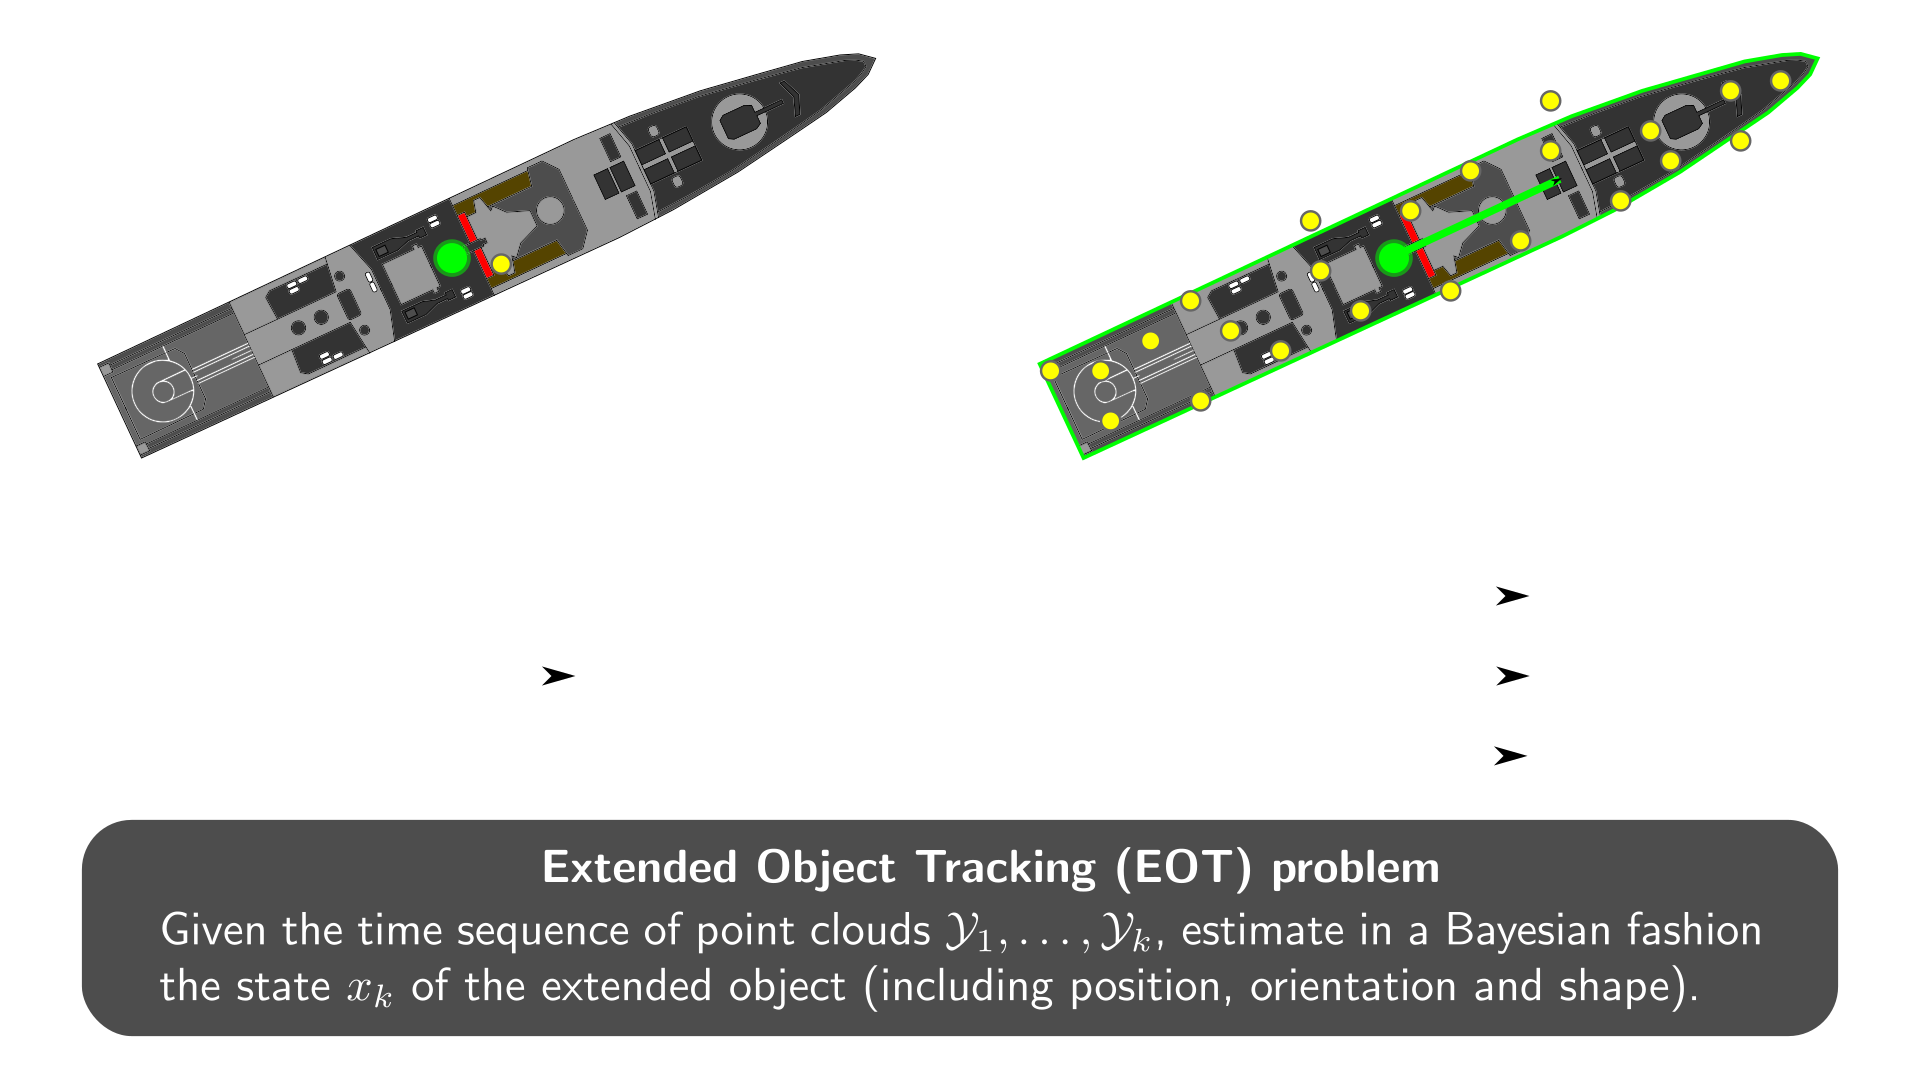
\includegraphics[width=1\textwidth]{Inkscape/potvseot.pdf}
\end{frame}

\begin{frame}{State of the art}
	\centering
	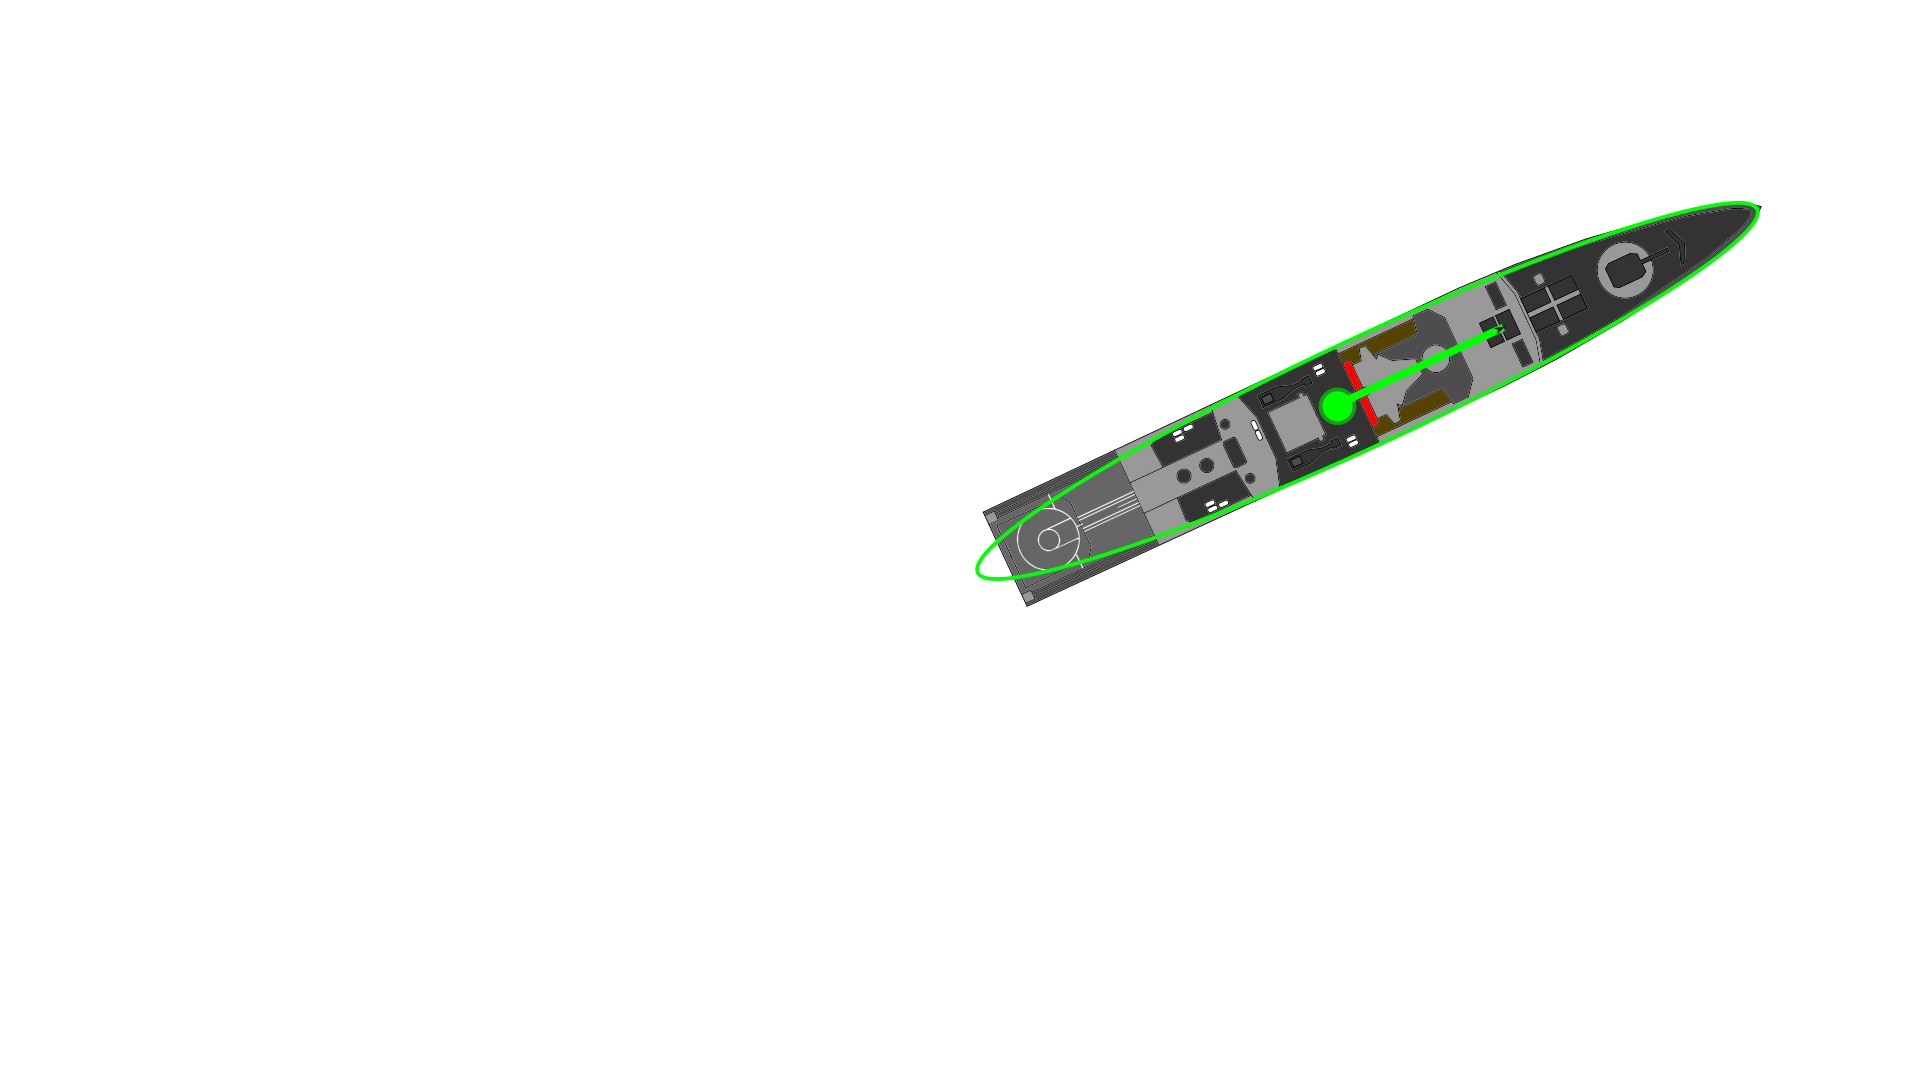
\includegraphics[width=1\textwidth]{Inkscape/RMM.pdf}
\end{frame}

\begin{frame}{State of the art}
	\centering
	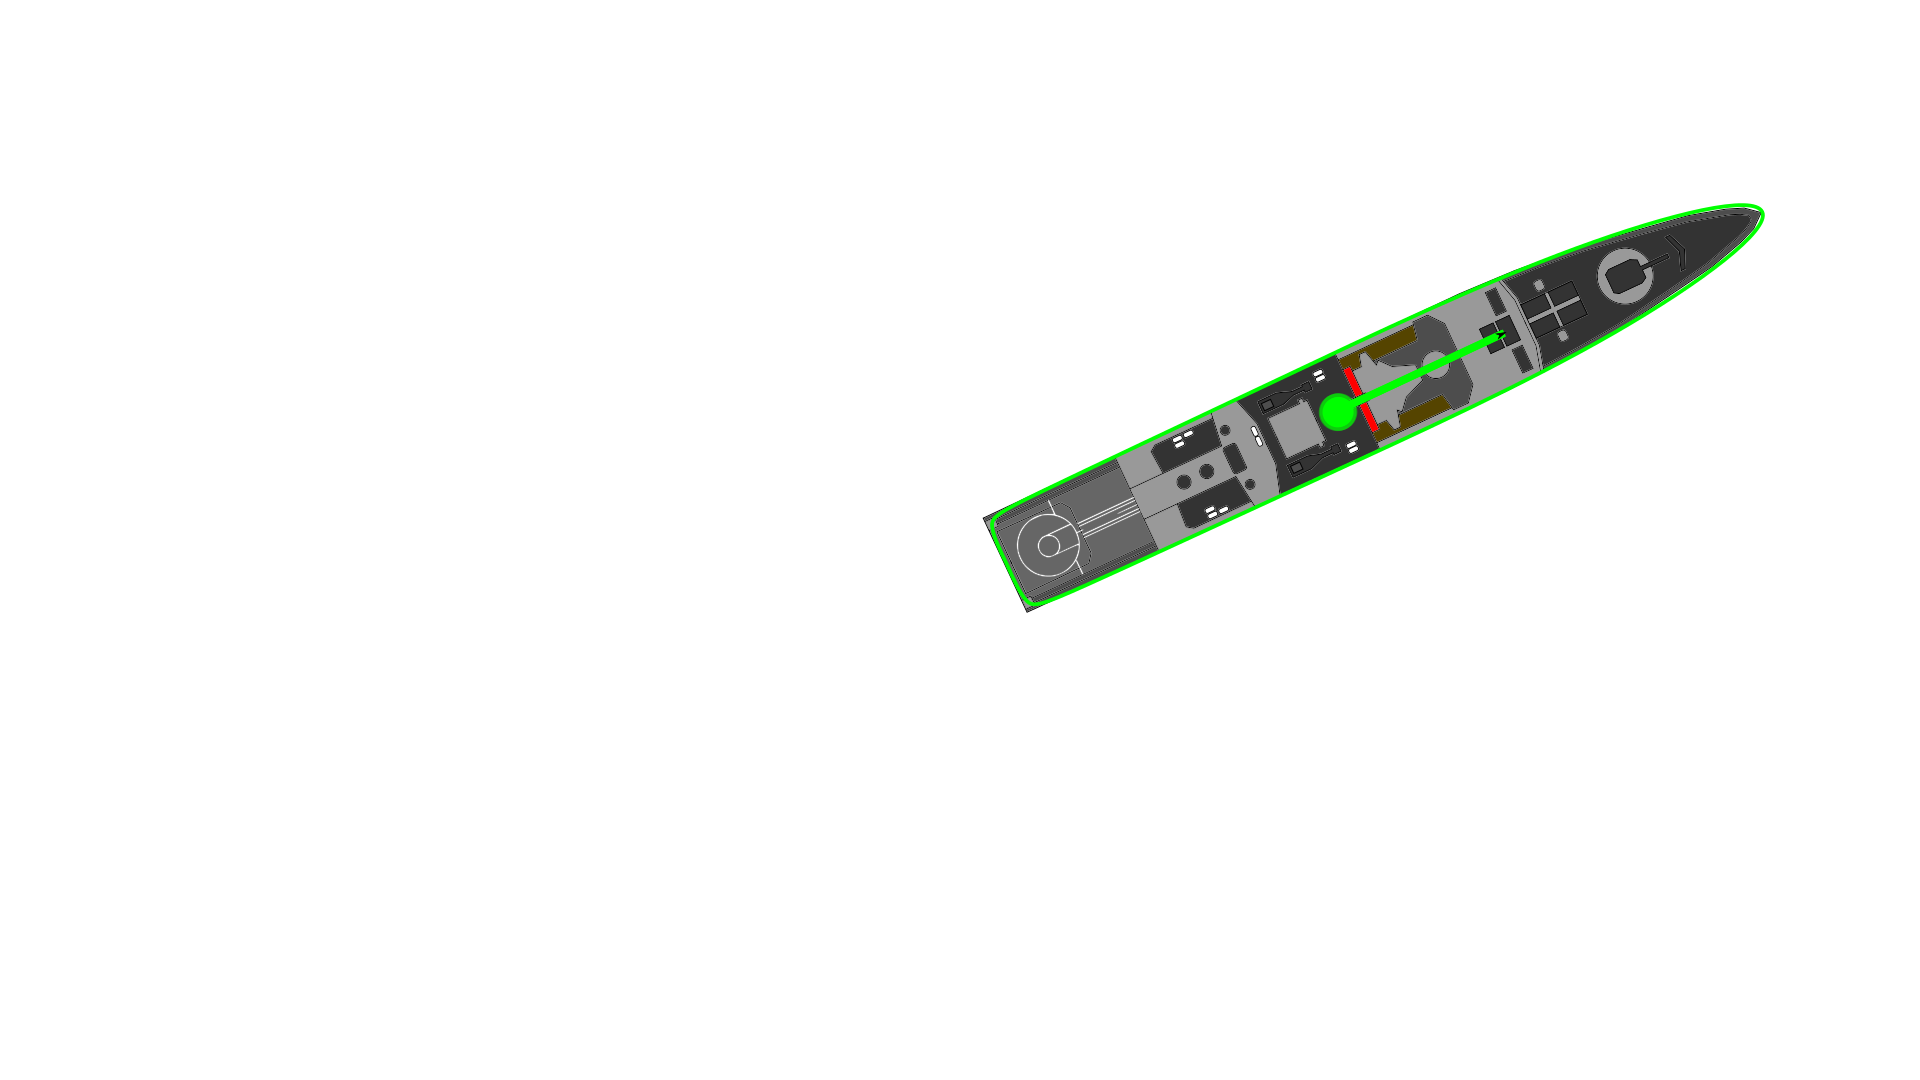
\includegraphics[width=1\textwidth]{Inkscape/RHM.pdf}
\end{frame}

\begin{frame}{Motivation}
	\begin{itemize}
	  \item\textbf{Maneuvering objects:} take advantage of the heading information to improve turning rate estimation in 
	  coordinated turn models (and their generalizations).
	  {\color{green}\textbf{PRO}}: discard interacting multiple models in prediction.\\
	  {\color{red}\textbf{CON}}: fragile to measurement noise.
	\end{itemize}
\end{frame}

\begin{frame}{Motivation}
	\begin{itemize}
	  \item\textbf{Efficient statistics:} 
		rather than process each point in $\mathcal{Y}=\{y_1,\dots,y_m\}$, process
		\begin{equation*}
			\begin{array}{ccc}
		  \overline y \triangleq \frac{1}{m}\sum_{j=1}^{m}y^{(j)}
		  & \phantom{+++} &
		  \overline Y \triangleq \frac{1}{m-1}\sum_{j=1}^{m}
		  \left(y^{(j)}-\overline y\right)
		  \left(y^{(j)}-\overline y\right)'\\[0.1cm]
		  \text{sample mean} & \phantom{+++} & \text{sample covariance}\\[0.1cm]
			\end{array}
		\end{equation*}
		to infer the object’s position $p$, heading $h$, length $2\ell_1$, width $2\ell_2$.\\
		{\color{green}\textbf{PRO}}: cheap computational cost.\\
		{\color{red}\textbf{CON}}: loss of information.
	\end{itemize}
\end{frame}

\begin{frame}{Motivation}  
	\begin{itemize}
	  \item\textbf{Shape classification:}  
		cast shape estimation as a classification problem over a known shape family (\textbf{shape library}).\\
		{\color{green}\textbf{PRO}}: arbitrarily complex shapes can be recognized.\\
		{\color{green}\textbf{PRO}}: robustness to occlusion.\\
		{\color{red}\textbf{CON}}: only known shapes can be handled.
	\end{itemize}
\end{frame}
  
  

\section[Tracking for maneuvering objects]{Tracking for maneuvering objects}

\begin{frame}{Tracking for maneuvering objects}  
	An object is \textbf{maneuvering} iff its speed $s(t)$ and/or turning rate $\omega(t)$ 
	vary in time.

	\begin{center}
		\includegraphics[width=0.9\textwidth]{Inkscape/maneuver.pdf}
	\end{center}
	\pause
	\textbf{(1)} such variables are useful to improve position and heading predictions.
	\pause
	\newline
	\textbf{(2)} in EOT, we can ``directly observe'' position and heading from data.
	\pause
	\newline
	\begin{center}
	\textbf{IDEA:} define a prediction model to estimate $s$, $\omega$ and their derivatives
	\end{center} 
\end{frame}

\begin{frame}{Tracking for maneuvering objects}
	\begin{center}
		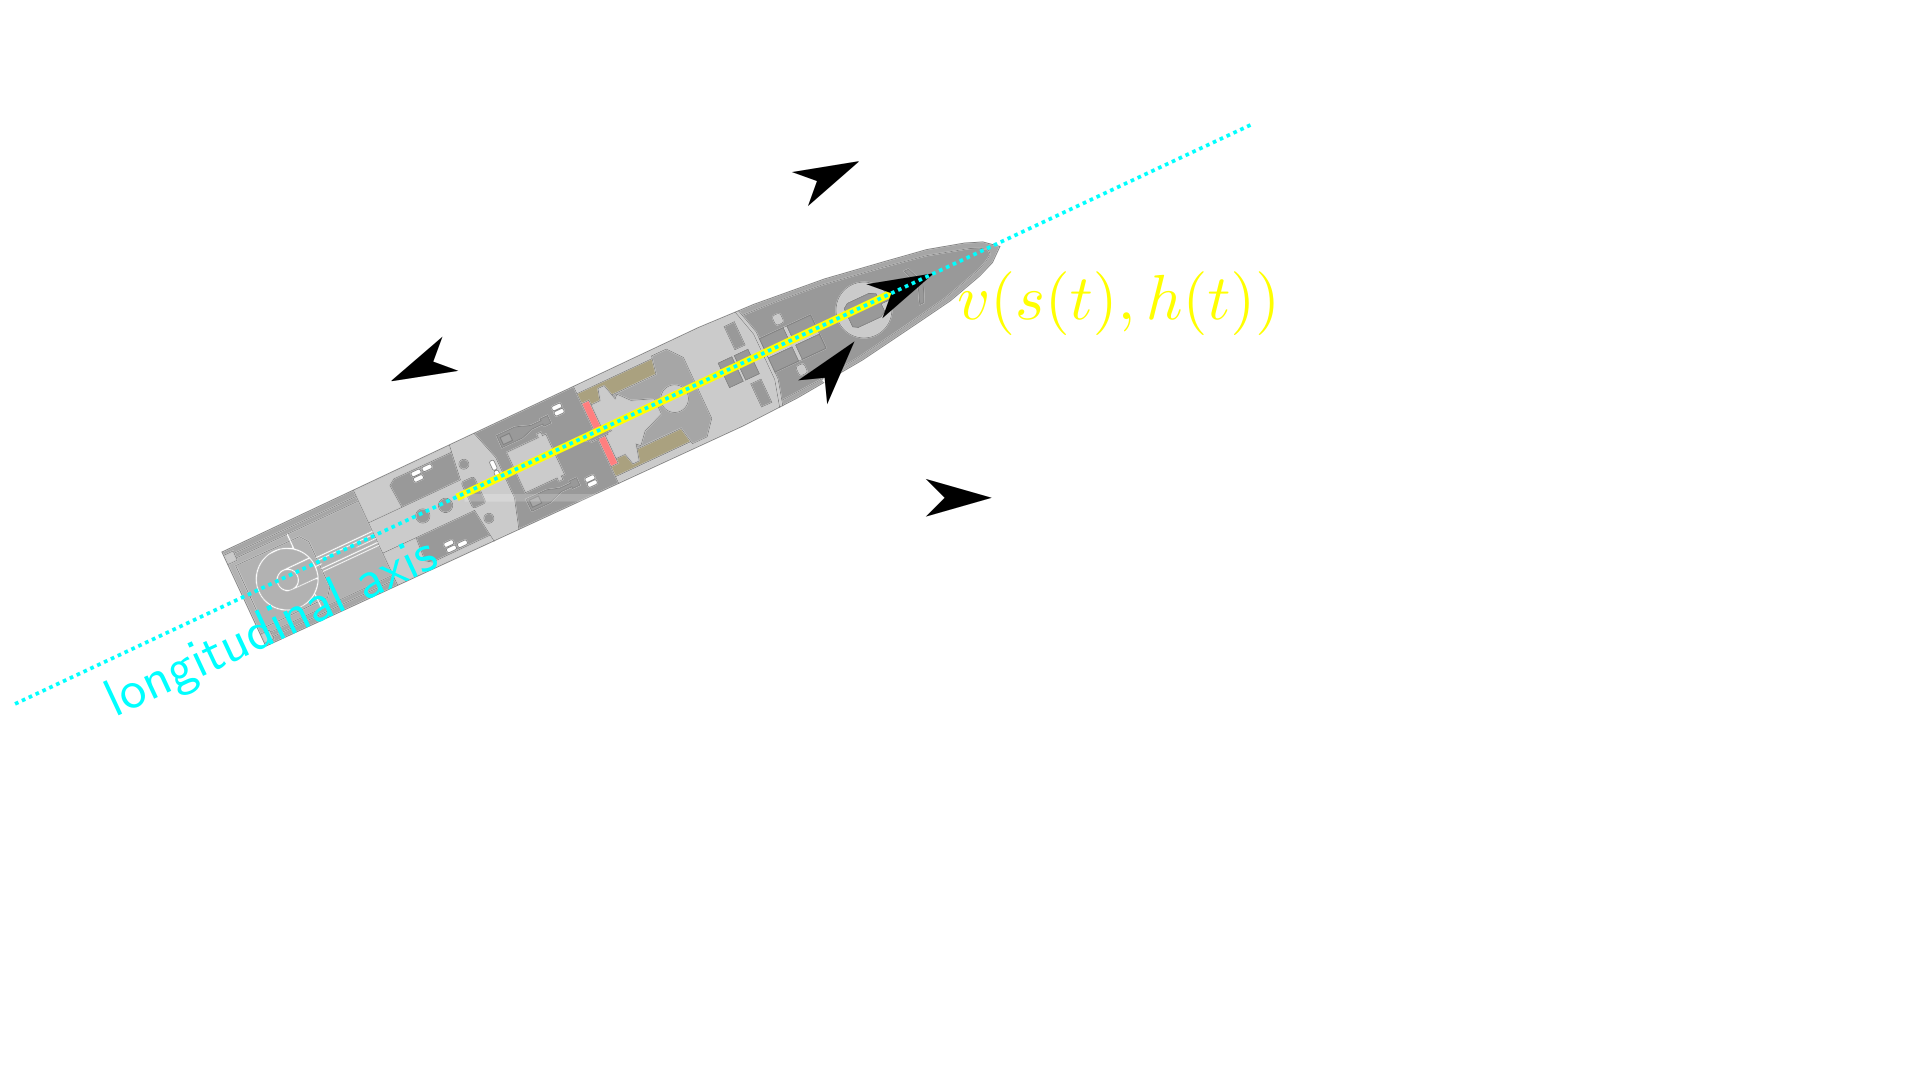
\includegraphics[width=1.0\textwidth]{Inkscape/nonholo.pdf}
	\end{center}
\end{frame}

\begin{frame}{Tracking for maneuvering objects}  
Kinematic state
\begin{equation*}
x\triangleq\left[\begin{array}{cc}
p' & \ell'
\end{array}\right]'
\qquad
\ell\triangleq\left[\begin{array}{ccccccc}
	h & s & \cdots & s^{(\Lambda-1)} & \omega & \cdots & \omega^{(O-1)}
	\end{array}\right]'
\end{equation*}
\pause
Dynamics discretization
\begin{equation*}
	\begin{aligned}
		\dot p(t) 	 &= f(\ell(t))\\
		\dot \ell(t) &= A\ell(t)
	\end{aligned}
\qquad \Rightarrow \qquad
\begin{aligned}
	p_{k}    &=p_{k-1} + \int_{(k-1)T}^{kT} v(\ell(\tau)) \text{ d}\tau \\
	\ell_{k} &=\exp(AT)\,\ell_{k-1}
\end{aligned}
\end{equation*}
\pause
$\varLambda:O$ prediction model
\begin{equation*}
\begin{aligned}
	p_{k}    &=p_{k-1} + T\,\frac{v(\ell_{k-1})+v(\ell_{k})}{2} + w_k^{p} \\
	\ell_{k} &=\exp(AT)\,\ell_{k-1}+w_k^{\ell}
\end{aligned}
\qquad w_k\sim\mathcal{N}(0,Q)
\end{equation*}
\end{frame}

\begin{frame}{Tracking for maneuvering objects}
$\varLambda:O$ predictor 
\vspace{-0.3cm}
\begin{equation*}
	\begin{aligned}
x_{k|k-1} &= \overline{f}_{k|k-1} \\
P_{k|k-1} &= F_{k|k-1}+Q
	\end{aligned}
\end{equation*}
where 
\begin{equation*}
\begin{aligned}
	f(x)&\triangleq \left[\begin{array}{c}p+T\frac{v(\ell)+v(\exp(AT)\ell)}{2};\quad \exp(AT)\ell
\end{array}\right]\\
\overline{f}_{k|k-1} &\triangleq \int f(x) \, \mathcal{N}(x;x_{k-1|k-1},P_{k-1|k-1}) \text{ d}x\\
F_{k|k-1} &\triangleq \int \left(f(x)-\overline{f}_{k|k-1}\right)\left(f(x)-\overline{f}_{k|k-1}\right)'\mathcal{N}(x;x_{k-1|k-1},P_{k-1|k-1}) \text{ d}x
\end{aligned}
\end{equation*}
and the integrals can be computed via:
\begin{itemize}
	\item linearization (EKF);
	\item Gaussian quadrature (e.g., UKF, CKF);
	\item or any other integration method (Grid integration, Importance Sampling, etc...).
\end{itemize}
\end{frame}

\begin{frame}{Tracking for maneuvering objects}
	\begin{center}
		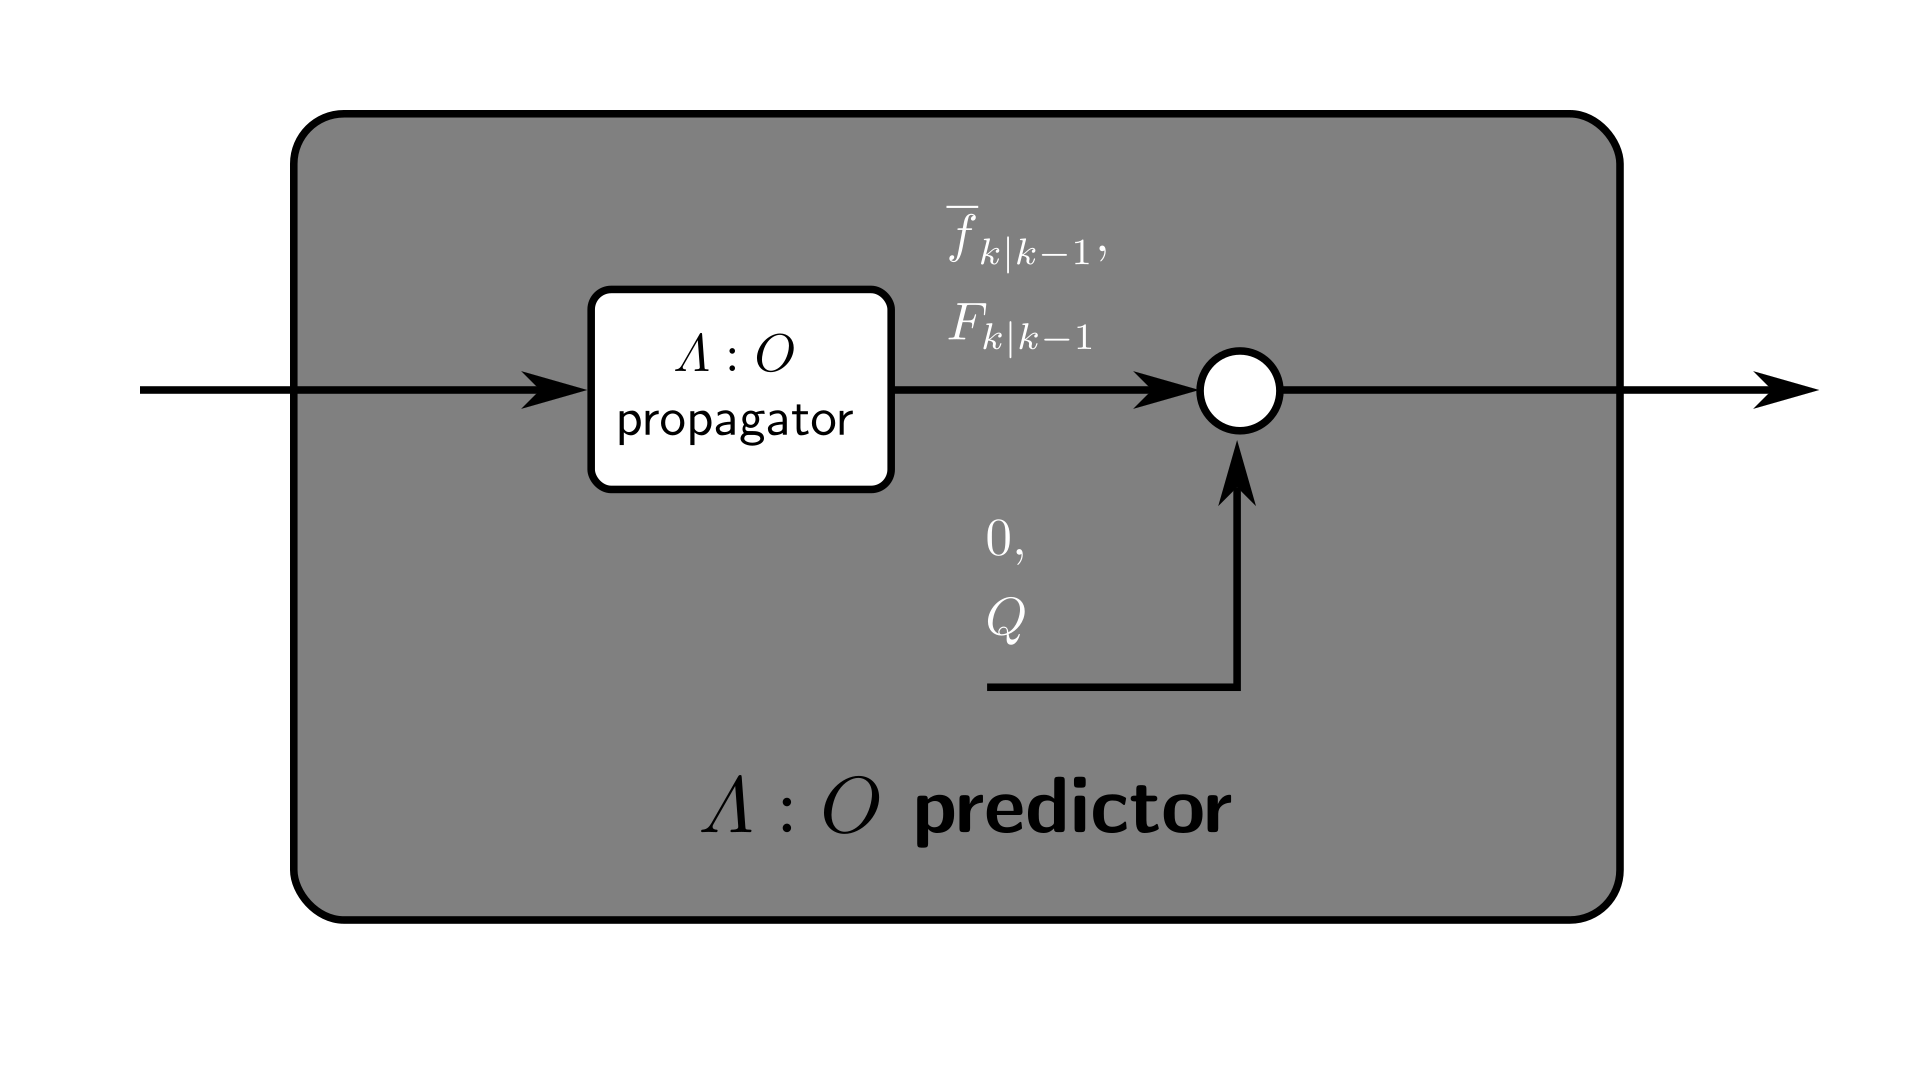
\includegraphics[width=1\textwidth]{Inkscape/LOpredictor.pdf}
	\end{center}
\end{frame}

\section[Tracking for elliptical objects]{Tracking for elliptical objects}

\begin{frame}{Tracking for elliptical objects}
	Multiplicative error model (MEM) [Baum]
	\begin{equation*}
		\begin{aligned}
			y&=p+U(h)\,D(e)\,q+v\\
			q &\sim \mathcal{N}(0,I/k)\\
			v &\sim \mathcal{N}(0,\sigma_v^2 I)
		\end{aligned}
		\qquad 
		\begin{aligned}
		U(h) &\triangleq \left[\begin{array}{cc}
		\cos h & - \sin h \\
		\sin h & \cos h
		\end{array}\right]\\
		D(e)&\triangleq 
		\left[\begin{array}{cc}
			a & 0 \\
			0 & b
			\end{array}\right]
		\end{aligned}
	\end{equation*}
	\pause
	Measurement distribution (given $p,h,\ell$)
	\begin{equation*}
	y \sim \mathcal{N}\left(p,\quad U(h)\,D\left(\left[\frac{a^2}{k}+\sigma_v^2;\qquad
	\frac{b^2}{k}+\sigma_v^2\right]\right)\,U(h)'\right)
	\vspace{-0.1cm}
	\end{equation*} 
	\begin{itemize}
		\item $k=2$ if we model a point cloud distributed over the object contour; 
		\item $k=4$ if we model a point cloud distributed over the object surface.
	\end{itemize}
	\pause
	\begin{center}
		\textbf{IDEA:} estimate $p$, $h$, $\ell$ \textit{directly} from $\overline{y}\approx p$, $\overline{Y}\approx \Sigma_y$
	\end{center}
\end{frame}

\begin{frame}{Tracking for elliptical objects}
\textbf{\textbf{QUESTION}:} what does it mean \textit{directly}?

\textbf{\textbf{ANSWER}:} we define the pseudo-measurement, called \textit{static estimate}, as   
\begin{equation*}
\mathbb{Y} \triangleq \left[\begin{array}{ccc}
\hat{p}' & \hat{h} & \hat{e}'
\end{array}\right]'
\end{equation*}
and its covariance
\begin{equation*}
\Sigma_{\mathbb{Y}} \triangleq \left[\begin{array}{ccc}
\Sigma_{\hat{p}} & \Sigma_{\hat{p}\hat{h}} & \Sigma_{\hat{p}\hat{e}} \\
\ast & \Sigma_{\hat{h}} & \Sigma_{\hat{h}\hat{e}} \\
\ast & \ast & \Sigma_{\hat{e}}
\end{array}\right]
\end{equation*}
\pause
Then we perform a \textit{one-shot} (!!!) Kalman correction based on $\overline{Y}$. 
\newline
\textbf{NOTE}: mixed terms $\Sigma_{\hat{p}\hat{h}}$, $\Sigma_{\hat{p}\hat{e}}$, $\Sigma_{\hat{h}\hat{e}}$ are neglected for simplicity.
\end{frame}

\begin{frame}{Tracking for elliptical objects}
	How do we compute the static estimates?
	\vspace{-0.2cm}
\begin{table}[h!]
\centering
\setlength{\tabcolsep}{12pt} 
\begin{tabular}{l@{\hspace{2cm}}l}
\pause
$\displaystyle 
\hat{p} \triangleq \overline{y}
$ 
& 
$\displaystyle 
\Sigma_{\hat{p}} = \frac{1}{m}\,\overline{Y}
$ 
\\[1.2em]
\pause
$\displaystyle 
\hat{h} \triangleq \frac{1}{2}\,\textrm{atan2}\left(2\overline{Y}_{12},\overline{Y}_1-\overline{Y}_2\right)
$
&
$\displaystyle 
\Sigma_{\hat{h}} = \frac{1}{m-1}\frac{\lambda_1\,\lambda_2}{(\lambda_1-\lambda_2)^2}
$
\\[1.2em]
$\displaystyle 
\hat{e} \triangleq \sqrt{k}
\begin{bmatrix}
\sqrt{\lambda_1-\sigma_v^2} \\[4pt]
\sqrt{\lambda_2-\sigma_v^2}
\end{bmatrix}
$
&
$\displaystyle 
\Sigma_{\hat{e}} = \frac{1}{m-1} \frac{k}{2}
\begin{bmatrix}
\frac{\lambda_1^2}{\lambda_1-\sigma_v^2} &
\frac{\lambda_1\lambda_2}{2\sqrt{(\lambda_1-\sigma_v^2)(\lambda_2-\sigma_v^2)}} \\[4pt]
\ast &
\frac{\lambda_2^2}{\lambda_2-\sigma_v^2}
\end{bmatrix}
$
\end{tabular}
	\vspace{0.2cm}
\end{table}
	where $\lambda_1$, $\lambda_2$ are the eigenvalues of $\overline{Y}=[\overline{Y}_1,\overline{Y}_{12};\ast, \overline{Y}_2]$ and $m$ is the cloud cardinality.
	\newline
	$\Sigma_{\hat{h}}$, $\Sigma_{\hat{e}}$ are obtained via first-order error propagation, i.e.
	\begin{equation*}
		\Sigma_{\chi} = \frac{\partial \chi}{\partial \textrm{vec}\overline{Y}} \, \Sigma_{\textrm{vec}\overline{Y}} \, \left(\frac{\partial \chi}{\partial \textrm{vec}\overline{Y}}\right)' 	\qquad \chi= \hat{h}, \hat{e}
	\end{equation*}
\end{frame}


\begin{frame}{Tracking for elliptical objects}
Recall 
\begin{equation*}
\Sigma_{\hat{h}} = \frac{1}{m-1}\frac{\lambda_1\,\lambda_2}{(\lambda_1-\lambda_2)^2}
\qquad
\Sigma_{\hat{\ell}} = \frac{1}{m-1} \frac{k}{2}
\begin{bmatrix}
\frac{\lambda_1^2}{\lambda_1-\sigma_v^2} &
\frac{\lambda_1\lambda_2}{2\sqrt{(\lambda_1-\sigma_v^2)(\lambda_2-\sigma_v^2)}} \\[4pt]
\ast &
\frac{\lambda_2^2}{\lambda_2-\sigma_v^2}
\end{bmatrix}
\end{equation*}
\pause
Implicit assumptions in Extended Object Tracking:
\begin{equation*}
\lambda_1 \gg \lambda_2 \gg \sigma_v^2
\end{equation*}
We can consider the margins $\lambda_1-\lambda_2$, $|\lambda_2-\sigma_v^2|$ as \textbf{quality indicators} of the Signal-to-Noise Ratio (SNR) characterizing the point cloud.
\end{frame}


\begin{frame}{Tracking for elliptical objects}
	Augmented $\varLambda:O$ state $x$ and static estimate $\mathbb{Y}$
	\begin{equation*}
	\begin{aligned}
	% x&\triangleq \left[\begin{array}{cccccccccc}
	% p' & h & s & \cdots & s^{(\Lambda-1)} & \omega & \cdots & \omega^{(O-1)} & e'
	% \end{array}\right]'\\
x&\triangleq\left[\begin{array}{cc}
p' & \ell'
\end{array}\right]'
\qquad
\ell\triangleq\left[\begin{array}{cccccccc}
	h & s & \cdots & s^{(\Lambda-1)} & \omega & \cdots & \omega^{(O-1)} & e'
	\end{array}\right]'\\
	\mathbb{Y} &\triangleq \left[\begin{array}{ccc}
	\hat{p}' & \hat{h} & \hat{e}' 
	\end{array}\right]'
	\end{aligned}
	\end{equation*}
	\pause
	Prediction equations (random walk for $e$)
	\begin{equation*}
		\begin{aligned}
		x_{k|k-1} &\triangleq \overline{f}_{k-1}\\
		P_{k|k-1} &\triangleq F_{k-1}+Q\\
		\end{aligned}
	\end{equation*}
	\pause
	Correction equations
	\begin{equation*}
	\begin{aligned}
		L_k&=P_{k|k-1} H' \left(H P_{k|k-1} H' + \Sigma_{\mathbb{Y}_k}\right)^{-1}\\
x_{k|k}&=(I-L_k H) x_{k|k-1}+L_k\,\mathbb{Y}_k\\
P_{k|k}&=(I-L_k H) P_{k|k-1}
\end{aligned}
\end{equation*}
\end{frame}

\begin{frame}{Tracking for elliptical objects}
	\begin{center}
		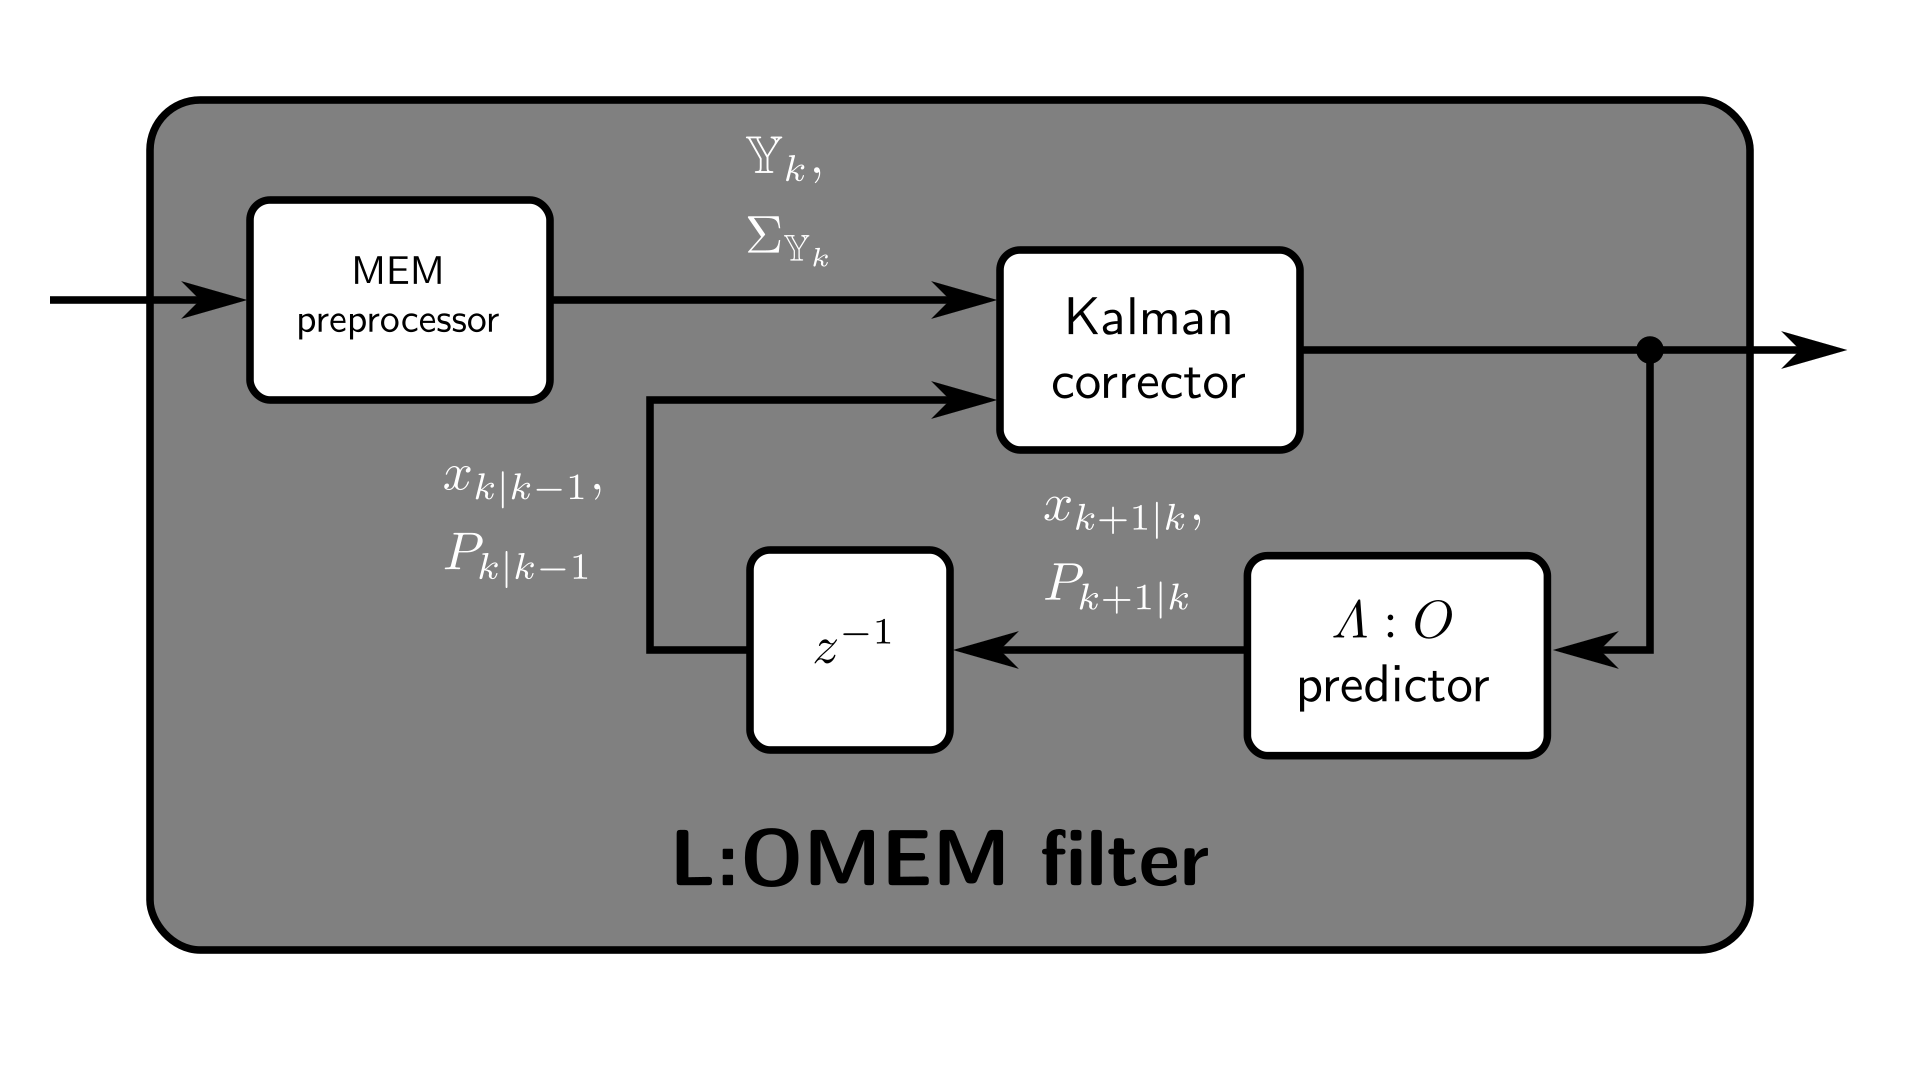
\includegraphics[width=0.95\textwidth]{Inkscape/LOMEM.pdf}
	\end{center}
\end{frame}

\begin{frame}{Tracking for elliptical objects}
Preprocessing has 2 main advantages over conventioal approaches:
\begin{itemize}
	\item \textbf{computational efficiency:} instead of processing $m$ points sequentially ($\mathcal{O}(m)$) or processing 
	a single stack of $m$ points ($\mathcal{O}(m^3)$), preprocessing reduces the correction to $\mathcal{O}(1)$;
	\pause
	\item \textbf{white box correction:} the static estimate $\mathbb{Y}_k$ is a subset of the object state $x_k$ and not a
	a nonlinear function $h(x)$ of it (as in RMM and RHM). Hence, we have "maximum correlation" $\Sigma_{x\mathbb{Y}}$ 
	between observation $\mathbb{Y}_k$ and state $x_k$.
\end{itemize}
\end{frame}

\section[Tracking for general objects]{Tracking for general objects}

\begin{frame}{Tracking for general objects}
Elliptic models are great for several reasons:
\begin{itemize}
\item Easy to implement and, more importantly, computationally cheap;
\item Allows for closed-form Bayesian updates \newline(+ simple multi-object, multi-sensor extensions);
\item They can classify objects with well-distinguished extensions.
\end{itemize}
\pause
However, in some scenarios they are deemed to fail:
\begin{itemize}
	\item When we have to distinguish objects with similar extensions;
	\item When we have to deal with \textbf{occlusions}.
\end{itemize}
\end{frame}

\begin{frame}{Tracking for general objects}
TODO: Elliptic fails picture
\end{frame}

\begin{frame}{Tracking for general objects}
	\textbf{QUESTION}: how do we overcome the limitations of elliptic models?
	\pause

	In many scenarios, we have \textbf{strong prior knowledge} about the object being tracked.
	\newline
	\pause
	We may know it is a car, ship, or aircraft; but not its specific manufacturing model.

	\vspace{1em}
	\pause
	\begin{center}
	\textbf{IDEA:} tackle shape estimation as a \textbf{classification} problem \newline(rather than a regression problem)
	\end{center}	

	\pause
	...moreover, it would be nice to keep the good features of elliptic models.
	\pause
\vspace{0.3cm}
\newline
	\textbf{Assumption:} we have at disposal a \textbf{shape library} of $C$ known "shapes" $c=1,..,C$.
\end{frame}

\begin{frame}{Tracking for general objects}
	\begin{center}
		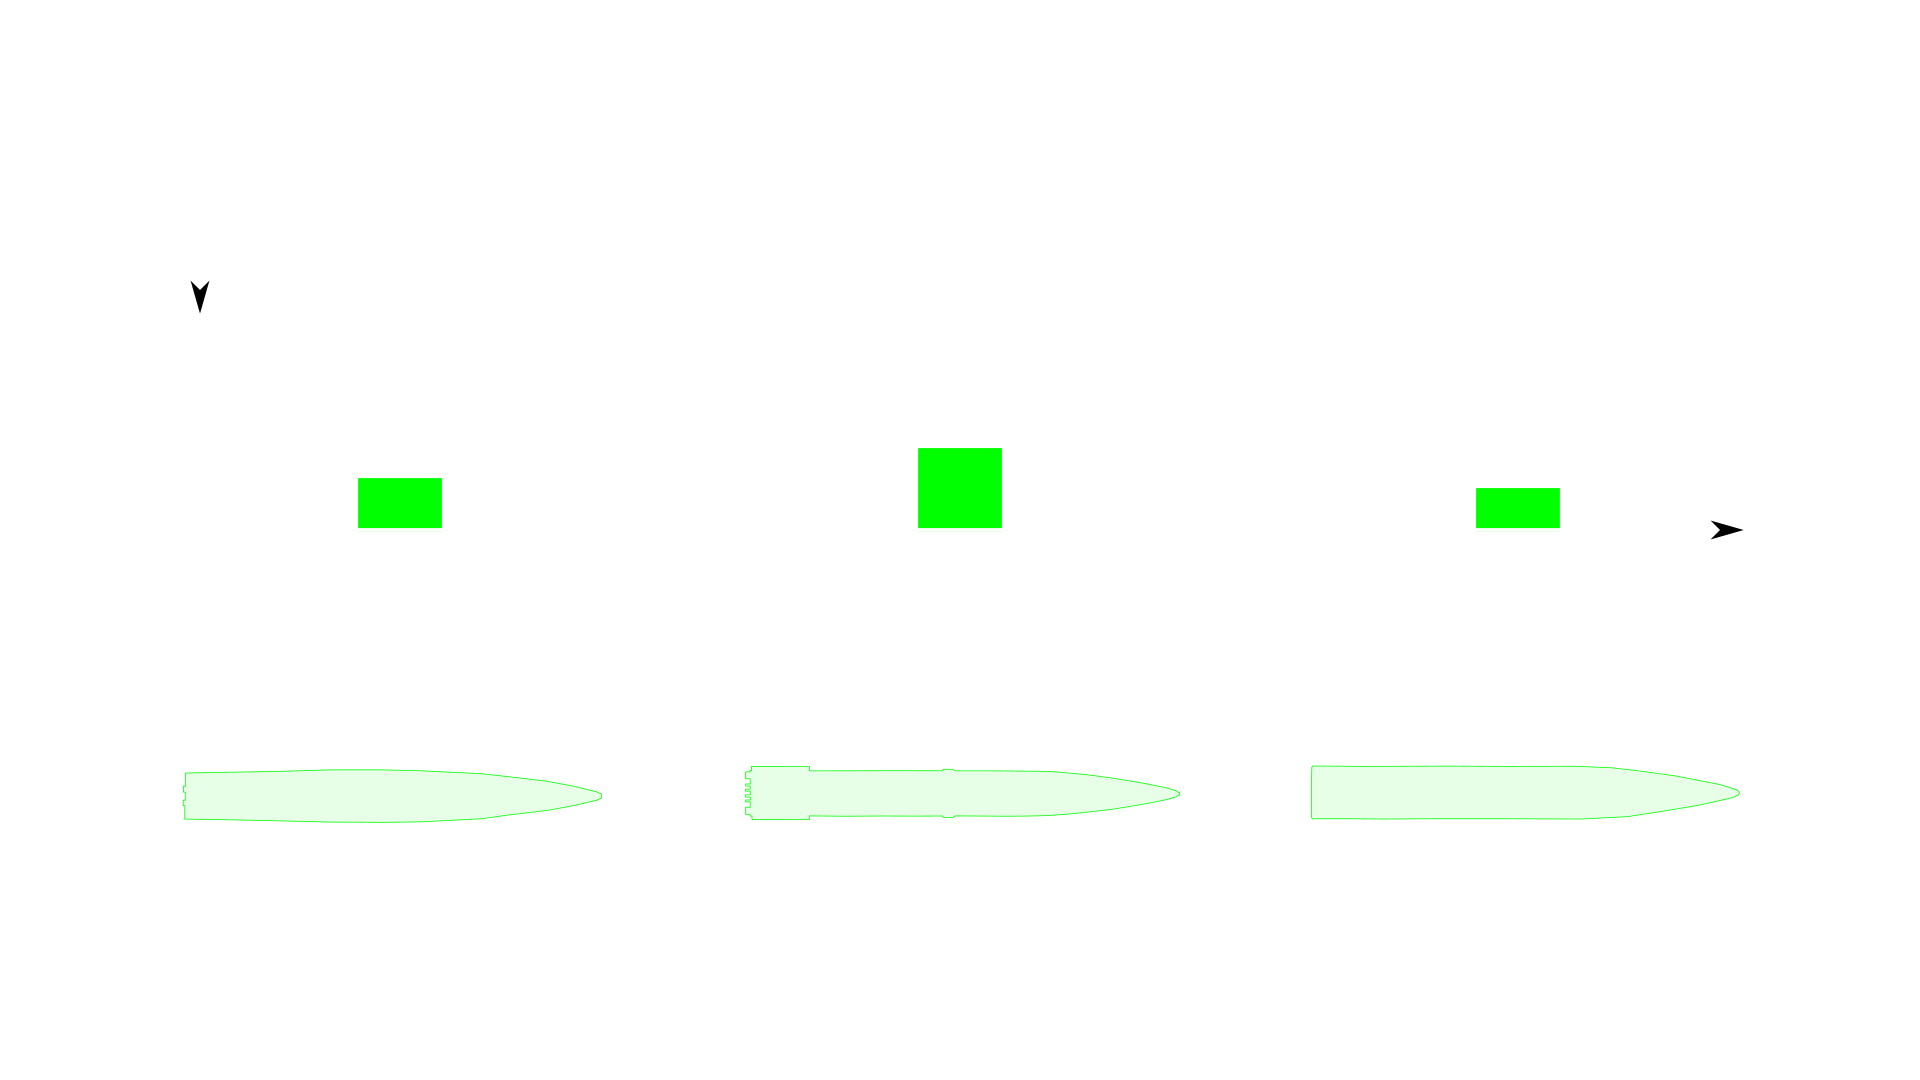
\includegraphics[width=1\textwidth]{Inkscape/classification.pdf}
	\end{center}
\end{frame}

\begin{frame}{Tracking for general objects}
Why not using Random Hypersurface Models?
\pause
\begin{itemize}
\item RHMs handle only star-convex shapes.
\item RHM-based filters employ Kalman filters (EKFs, UKFs) including in the state vector $n$ Fourier coefficients, or $n$ radius points, or $n$ vertex positions.
\begin{equation*}
	\textsf{RHM regression:}\quad \mathcal{O}(n^3)\end{equation*}
\item Typically, we use the estimated shape by RHM filters to classify tracked objects.
\newline Why not directly perform classification?
\end{itemize}
\end{frame}

\begin{frame}{Tracking for general objects}
Hybrid L:OMEM state
\begin{equation*}
\boldsymbol{x}\triangleq\left[\begin{array}{cc}
x' & c
\end{array}\right]'
\qquad\begin{aligned}
x&\triangleq\left[\begin{array}{ccccccccc}
	p' & h & s & \cdots & s^{(\varLambda-1)} & \omega & \cdots & \omega^{(O-1)} & e'
	\end{array}\right]'\\
c&\in\{1,\dots,C\}
\end{aligned}
\end{equation*}
\newline
Joint tracking and classification belief
\begin{equation*}
\begin{aligned}
\pi(\boldsymbol{x})&\triangleq \pi(x,c) = \underbrace{\pi^{x}(x)}_{\text{kinematic belief}}\,\underbrace{\pi^{c}(c|x)}_{\text{shape belief}}
\end{aligned}
\end{equation*}
\pause
\textbf{Track-to-Shape (T2S) filter} 
\begin{itemize}
	\item employs a \textit{tracker}\footnote{not necessarily L:OMEM} to update $\pi^{x}(x)$ according to data;
	\item employs a \textit{shaper} to update $\pi^{c}(c|x)$ according to data	.
\vspace{0.5cm}
\end{itemize}
\end{frame}

\begin{frame}{Tracking for general objects}
	\begin{center}
		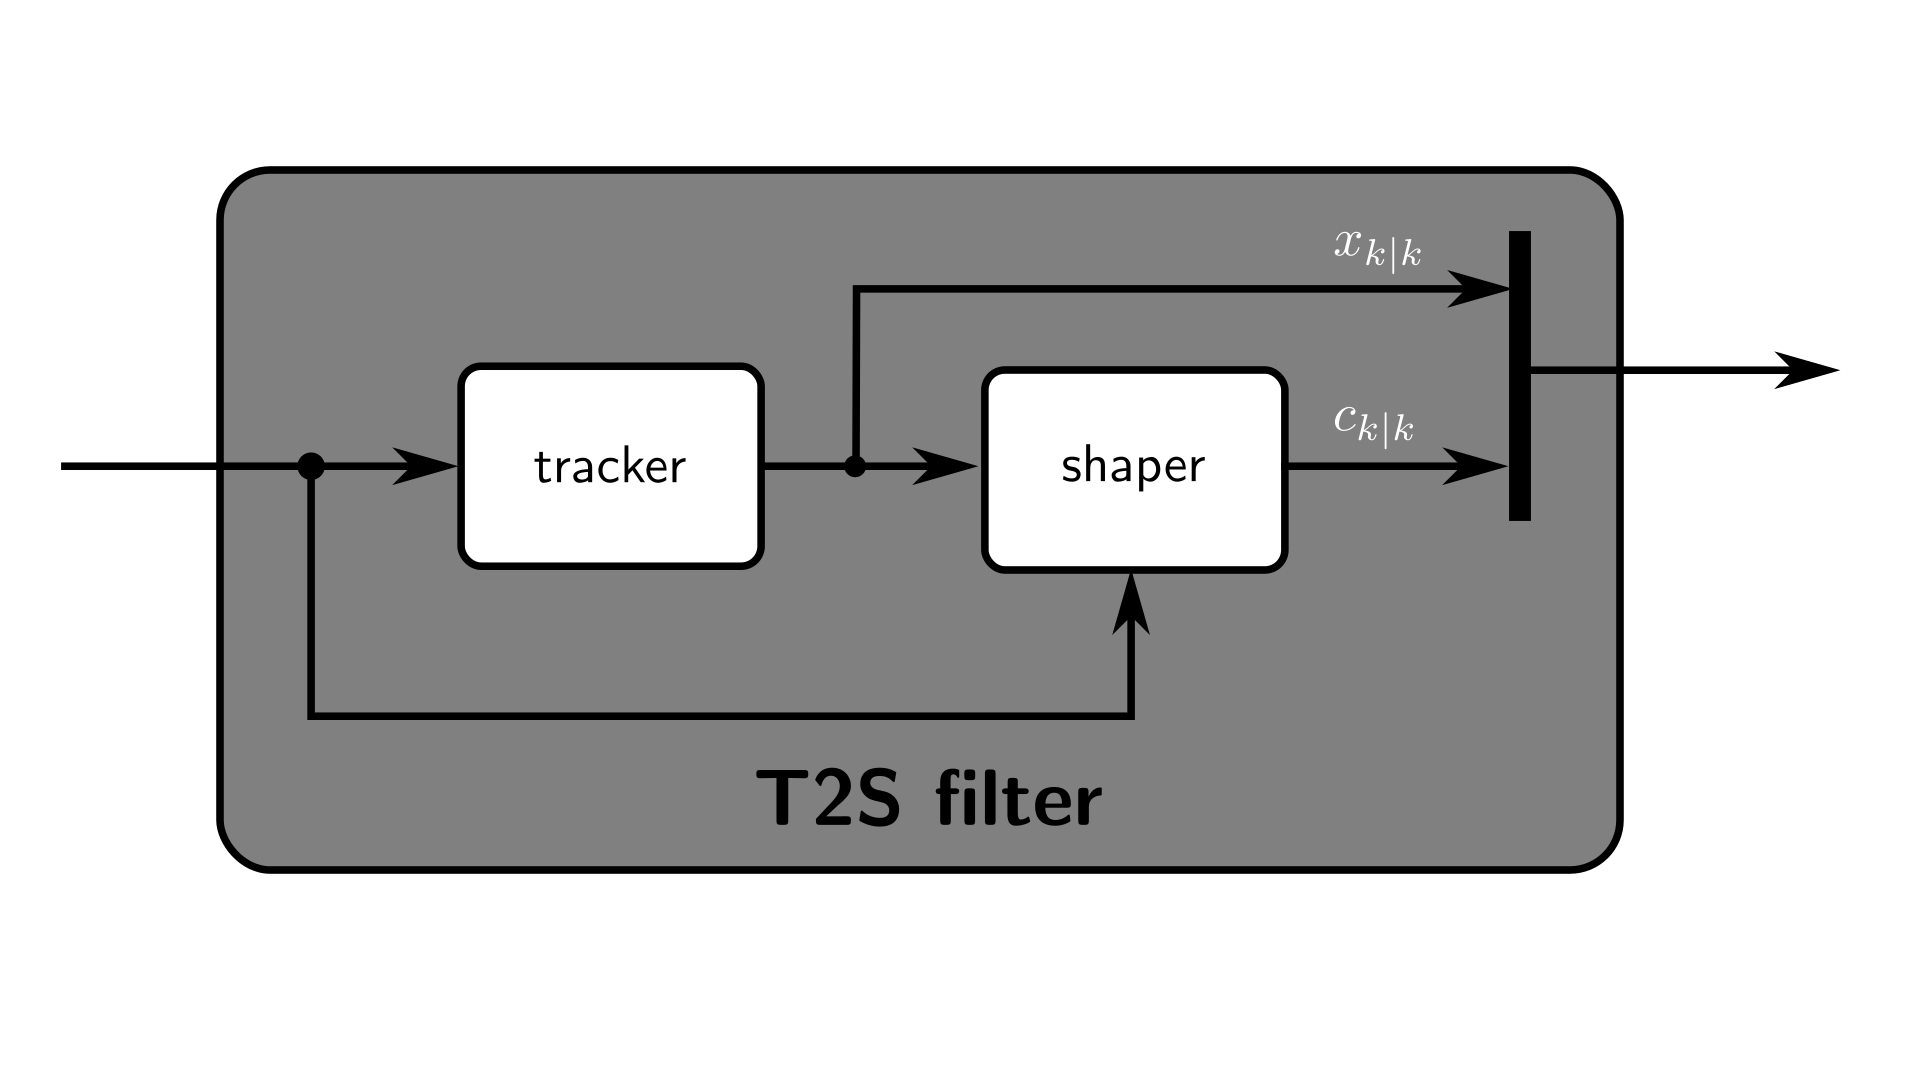
\includegraphics[width=1\textwidth]{Inkscape/T2S.pdf}
	\end{center}
\end{frame}

\begin{frame}{Tracking for general objects}
\textbf{QUESTION}: what is the "shape" of an object?

\pause
A reasonable definition of "shape" should uniquely depend on the object geometry.
\pause
\newline
We look for a definition that is:
\begin{itemize}
	\item invariant to translation;
	\item invariant to rotation;
	\item invariant to scale.
\end{itemize}
and generalizes the elliptic model and the RHM model.
\vspace{0.5cm}
\newline
\pause
Accordingly, we define the \textit{object shape} as a closed and non self-intersecting 
polygon contained in the unit square $[-0.5,+0.5]^2$. 
\newline Such polygon is defined by a \textbf{shape vector} $\widetilde{S}$ stacking the vertex coordinates.
\end{frame}

\begin{frame}{Tracking for general objects}
	\begin{center}
		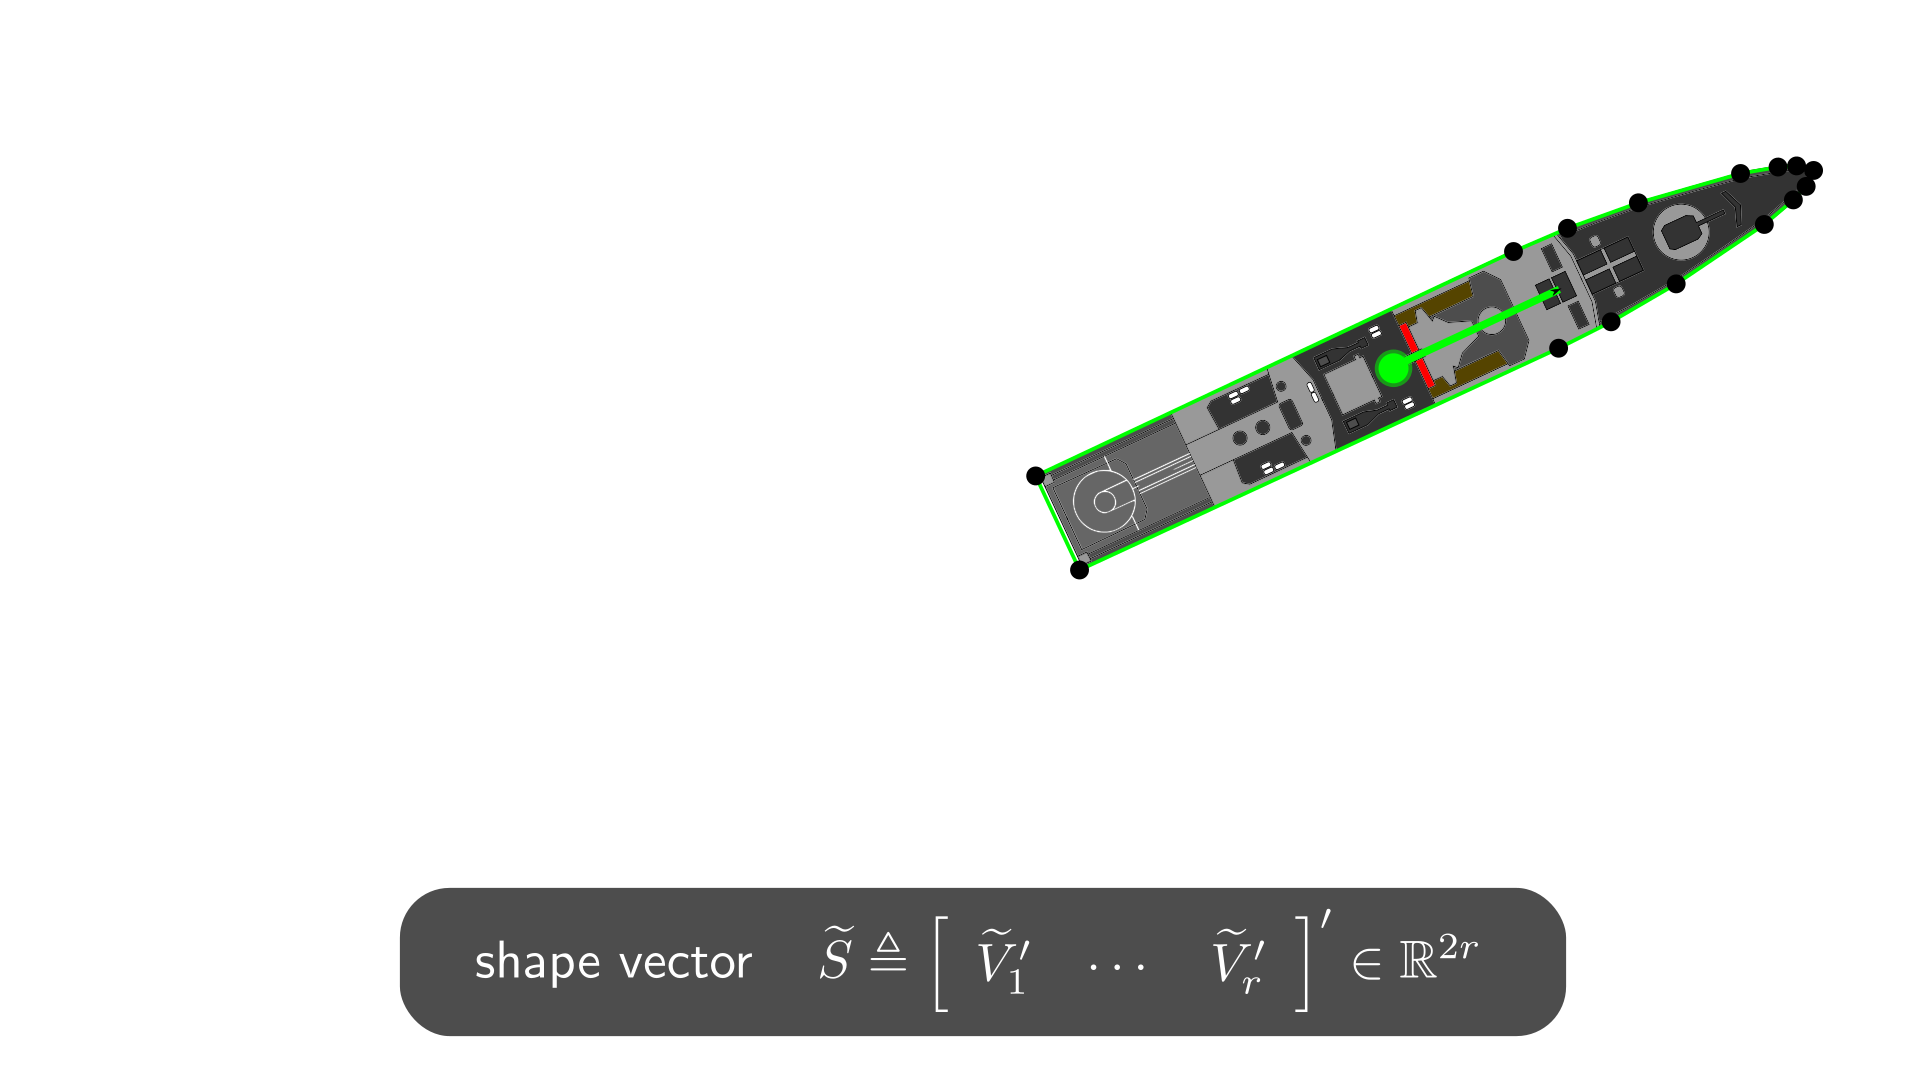
\includegraphics[width=1\textwidth]{Inkscape/LSM.pdf}
	\end{center}
\end{frame}

\begin{frame}{Tracking for general objects}
	Since the shape library $\{\widetilde{S}^{(c)}\}_{c=1}^C$ is defined over the unit square $[-0.5,+0.5]^2$, 
	we need to \textbf{whiten} the measurements before feeding them to the shaper.

	\pause
	This is an operation based on the output of the tracker
	\begin{equation*}
	\widetilde{\mathcal{Y}}\triangleq \{\widetilde{y}^{(j)}\}_{j=1}^m  
	\qquad
	\widetilde{y}^{(j)}\triangleq \left(U(\hat{h})\,D(\hat{e})\right)^{-1}\,\left(y^{(j)}-\hat{p}\right)
	\end{equation*}

	\pause
	Once whitened, the pointcloud can be compared to the shapes in the library via a \textbf{Bayesian classifier}, composed of:
	\begin{itemize}
	\item \textbf{(1)} an \textbf{Anti-Chattering} (AC) estimator.
	\item \textbf{(2)} a \textbf{Chapman-Kolmogorov} (CK) prediction step based on some suitable transition matrix;
	\item \textbf{(3)} a \textbf{Generalized Bayesian} (GB) correction step based on some suitable Pointcloud-to-Shape (PC2S) likelihood function;
	\end{itemize}
\end{frame}

\begin{frame}{Tracking for general objects}
	\begin{center}
		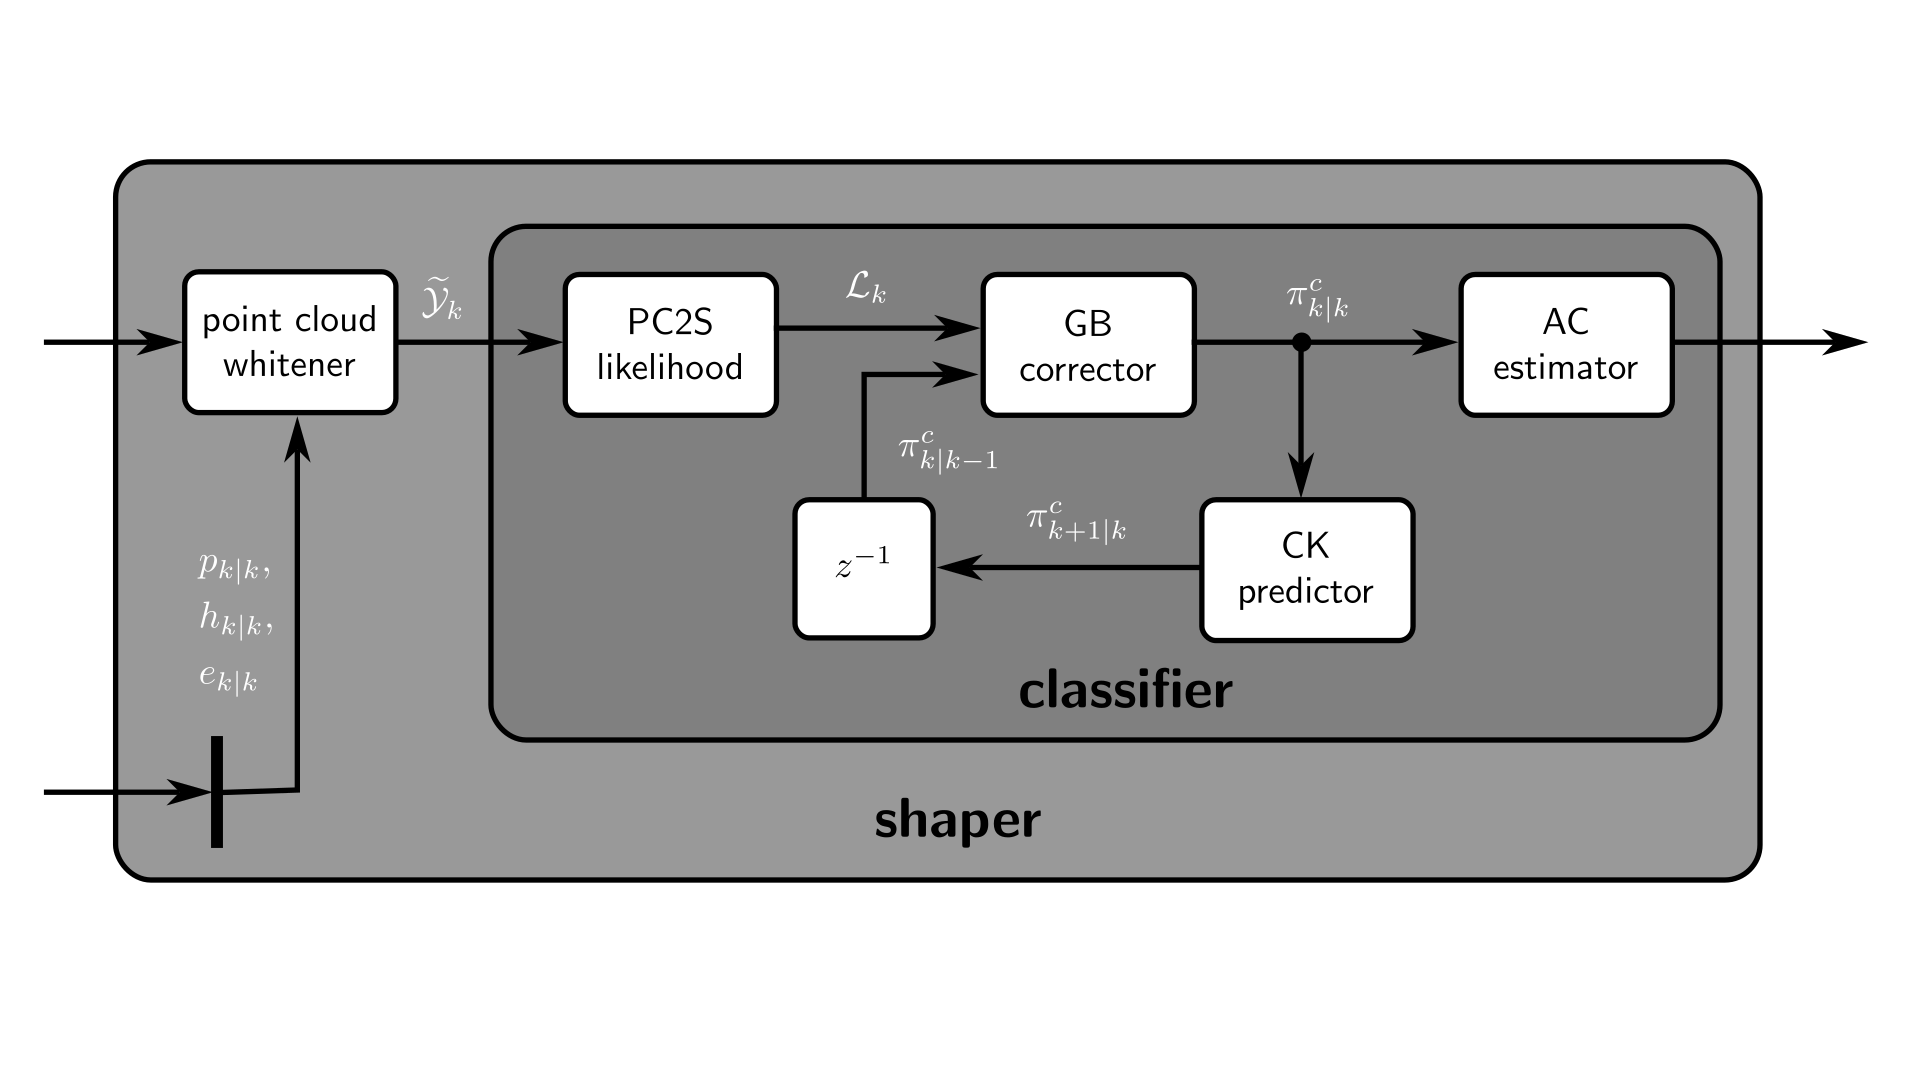
\includegraphics[width=1\textwidth]{Inkscape/shaper.pdf}
	\end{center}
\end{frame}

\begin{frame}{Tracking for general objects}
Notations
\begin{equation*}\begin{aligned}
\pi^{c} &\triangleq \left[\begin{array}{ccc}
\pi^{c}(1|x) & \cdots & \pi^{c}(C|x)
\end{array}\right]'\\
\mathcal{L} &\triangleq \textrm{diag}\left(
\mathcal{L}(\widetilde{\mathcal{Y}}| \widetilde{S}^{(1)}),\dots,
\mathcal{L}(\widetilde{\mathcal{Y}}| \widetilde{S}^{(C)})
\right)
\end{aligned}
\end{equation*}
\pause
\textbf{Chapman-Kolmogorov prediction}
\begin{equation*}
\pi_{k|k-1}^{c} = \mathcal{T} \,\pi_{k-1|k-1}^{c}
\end{equation*}
for a suitable transition matrix  $\mathcal{T}$.
\vspace{0.3cm}
\pause
\newline
\textbf{Generalized Bayesian correction}
\begin{equation*}
\pi_{k|k}^{c} \propto \mathcal{L}_k^{\frac{1}{\tau}}\,\pi_{k|k-1}^{c}
\end{equation*}
for a suitable temperature parameter $\tau>0$ and a suitable PC2S likelihood matrix $\mathcal{L}$.
\end{frame}

\begin{frame}{Tracking for general objects}
\textbf{(1) AC estimator}
\begin{equation*}
\pi_{k|k}^{c} = \mathcal{A} \,\pi_{k|k-1}^{c}
\end{equation*}
this estimator smooths out frequent changes in the Maximum A Posteriori (MAP) class estimate.
\end{frame}

\begin{frame}{Tracking for general objects}
	\textbf{(2) Transition matrix}
	\begin{equation*}
	\mathcal{T} \triangleq (1-\lambda)\,\mathcal{S} + \lambda\,\mathcal{R}
	\end{equation*}
	where $\lambda\in(0,1)$ is a forgetting factor and: 
	\begin{itemize}
		\item \textbf{similarity matrix}
		\begin{equation*}
			[\mathcal{S}]_{ij}\triangleq \textrm{sim}\left(\widetilde{S}^{(i)},\widetilde{S}^{(j)}\right) 
		\end{equation*}
		This term makes the classifier robust against geometric ambiguities between similar shapes. 
		Examples of similarity metrics are complementary Hausdorff distance, chamfer distance, earth mover distance, etc...
		\item \textbf{regularization matrix}
		\begin{equation*}
			[\mathcal{R}]_{ij}\triangleq \frac{1}{C}
		\end{equation*}
		This term makes the classifier robust against underflow issues.
	\end{itemize}
\end{frame}

% \begin{frame}{Tracking for general objects}
% 	\begin{center}
% 		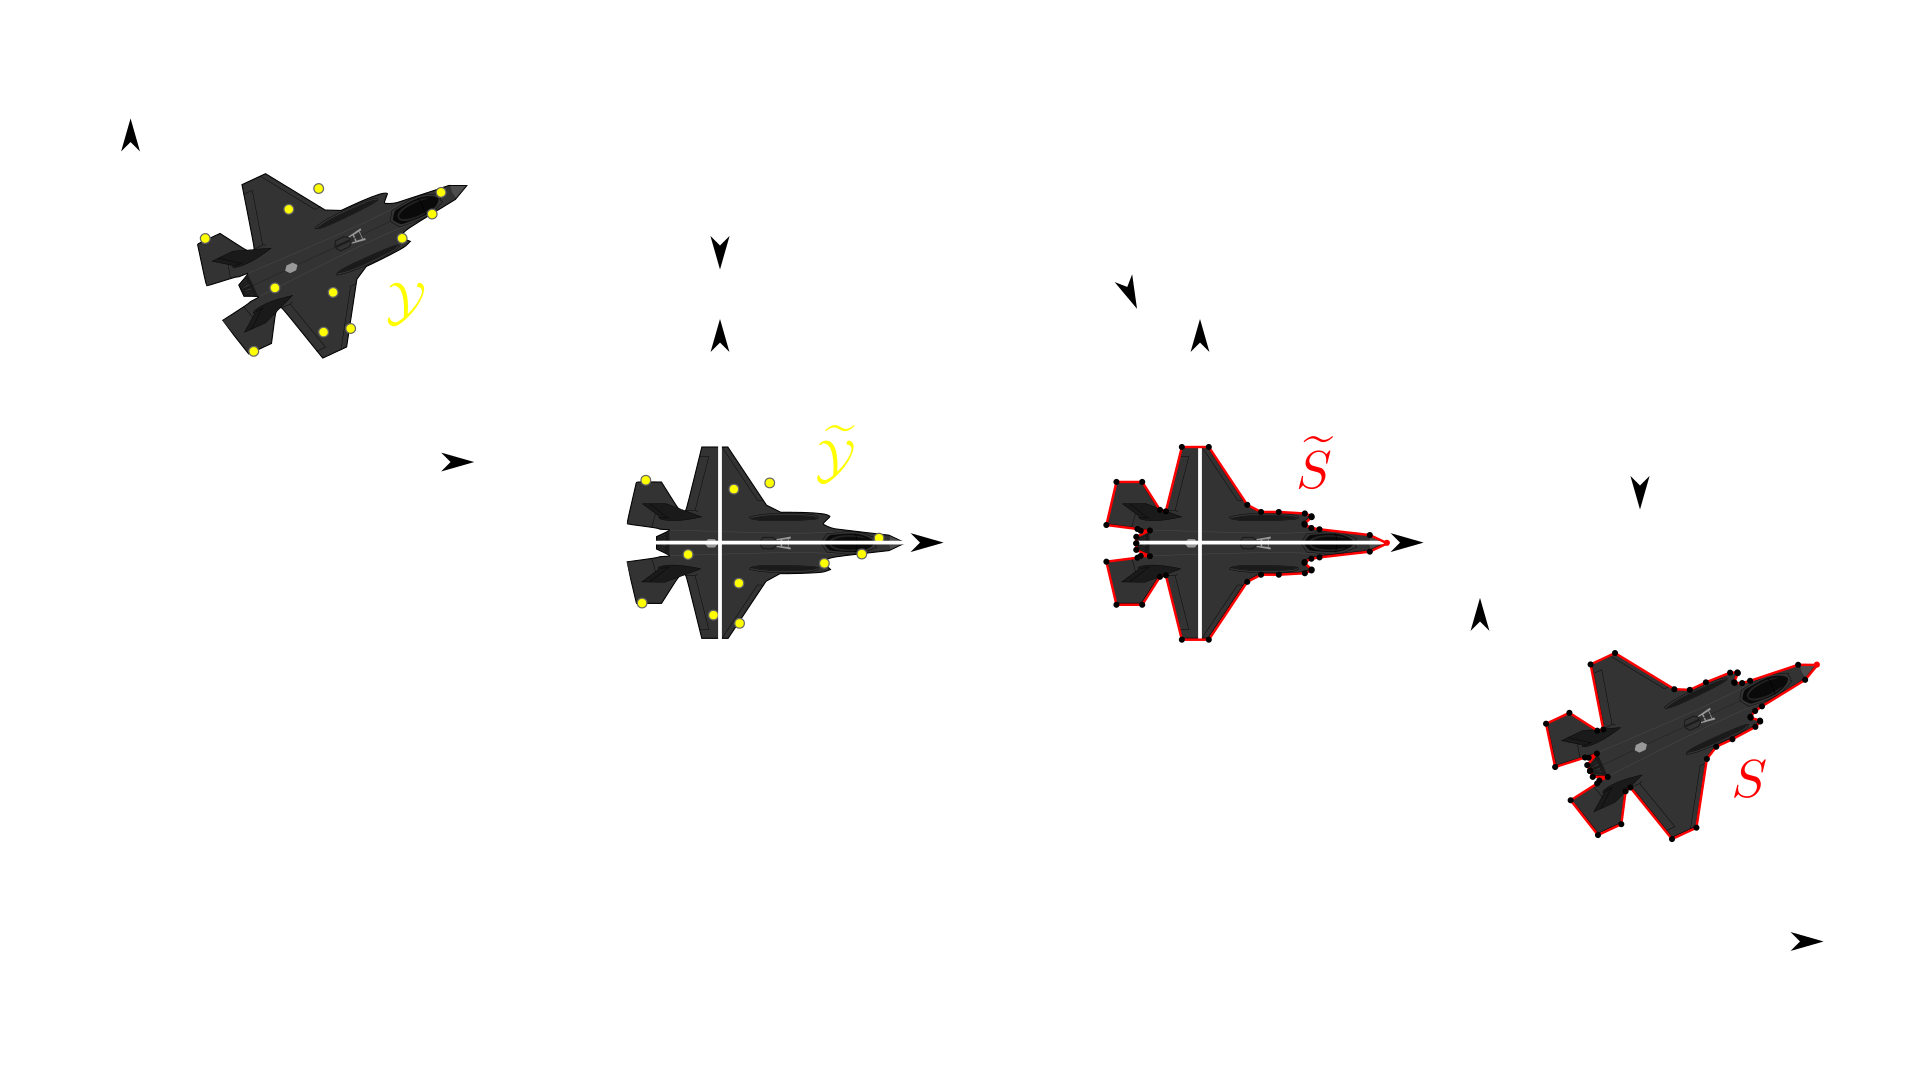
\includegraphics[width=1\textwidth]{Inkscape/whitening.pdf}
% 	\end{center}
% \end{frame}



% \begin{frame}{Tracking for general objects}
% 	Chapman-Kolmogorov predictor
% 	\begin{equation*}
% 	\pi_{k|k-1}(c)\triangleq (1-\lambda)\,\pi_{k-1|k-1}(c)+\lambda\,u(c)
% 	\end{equation*}
% 	\pause
% 	Bayes corrector
% 	\begin{equation*}
% 		\pi_{k|k}(c)\triangleq 	
% 		\frac{\mathcal{L}\left(\widetilde{\mathcal{Y}}_{k}|\widetilde{S}^{(c)}\right)\,\pi_{k|k-1}(c)}
% 		{\sum_{\nu}\mathcal{L}\left(\widetilde{\mathcal{Y}}_{k}|\widetilde{S}^{(\nu)}\right)\,\pi_{k|k-1}(\nu)}
% 	\end{equation*}
% 	\pause
% 	MAP estimator
% 	\begin{equation*}
% 		\begin{aligned}
% 	c_{k|k}&\triangleq \arg\max_{c} \pi_{k|k}(c)
% 	\end{aligned}
% 	\end{equation*}
% 	\pause
% 	\begin{center}
% 		\textbf{PROBLEM:} suitably define a likelihood function 
% 		$\mathcal{L}\left(\widetilde{\mathcal{Y}}|\widetilde{S}\right)$
% 	\end{center}
% \end{frame}

\begin{frame}{Tracking for general objects}
\textbf{(3) PC2S likelihood}
\begin{equation*}
\mathcal{L}\left(\widetilde{\mathcal{Y}}\,\big|\,\widetilde{S}^{(c)}\right)\triangleq 
\mathcal{L}^{\textrm{C}}\left(|\widetilde{\mathcal{Y}}|\,\big|\,\widetilde{S}^{(c)}\right)
\prod_{\widetilde{y}\in \widetilde{\mathcal{Y}}}\mathcal{L}^{\textrm{S}}
\left(\widetilde{y}\,\big|\widetilde{S}^{(c)}\right)
\end{equation*}
where:
\begin{itemize}
	\item $\mathcal{L}^{\textrm{C}}\left(|\widetilde{\mathcal{Y}}|\,\big|\,\widetilde{S}^{(c)}\right)$ is the \textbf{cardinality likelihood}. 
	\newline 
	It provides a cheap pre-screening of unlikely shapes based on the number of points in the cloud;
	\item $\mathcal{L}^{\textrm{S}}\left(\widetilde{y}\,\big|\widetilde{S}^{(c)}\right)$ is the \textbf{spatial likelihood}. 
	\newline
	It provides a deep analysis of the compatibility between each point in the cloud and the shape under test.
\end{itemize}

\pause
Accordingly, the pointcloud $\widetilde{\mathcal{Y}}$ is modeled as an \textbf{Independent and Identically Distributed Cluster (IIDC)} Random Finite Set. 
\end{frame}

\begin{frame}{Tracking for general objects}
Measurement model (surface)
\begin{equation*} 
\begin{aligned}
	\widetilde y&\triangleq \widetilde{z}+v\\
	\widetilde{z}&\sim \mathcal{U}(\widetilde{\mathcal{I}})\\
	v&\sim \mathcal{N}(0,R)
	\end{aligned}
\qquad \widetilde{\mathcal{I}}\triangleq \text{object surface}
\end{equation*}
\pause
Single point and point-cloud likelihoods 
\begin{equation*}
	\begin{aligned}
\mathcal{L}_{\text{s}}(\widetilde{y}|\widetilde{S})&\triangleq\int \mathcal{N}(\widetilde{y}-\widetilde{z};0,R)\,\,\mathcal{U}(\widetilde{z};\widetilde{\mathcal{I}})\,\text{ d}\widetilde{z}\\
\mathcal{L}_{\text{s}}(\widetilde{\mathcal{Y}}|\widetilde{S})&\triangleq\prod_{j=1}^{m}\mathcal{L}_{\text{s}}\left(\widetilde{y}^{(j)}|\widetilde{S}\right)
\end{aligned}
\end{equation*}
\pause
Uniform scattering distribution
\begin{equation*}
	\mathcal{U}(z;\widetilde{\mathcal{I}})\triangleq 
	\frac{\mathds{1}_{\widetilde{\mathcal{I}}}(z)}{\int_{\widetilde{\mathcal{I}}}
	\text{ d}\zeta}=\frac{\mathds{1}_{\widetilde{\mathcal{I}}}(z)}{\textrm{area}(\widetilde{\mathcal{I}})}
\end{equation*}
\end{frame}

\begin{frame}{Tracking for general objects}
	\begin{columns}[c] 
	  \column{0.45\textwidth}
	  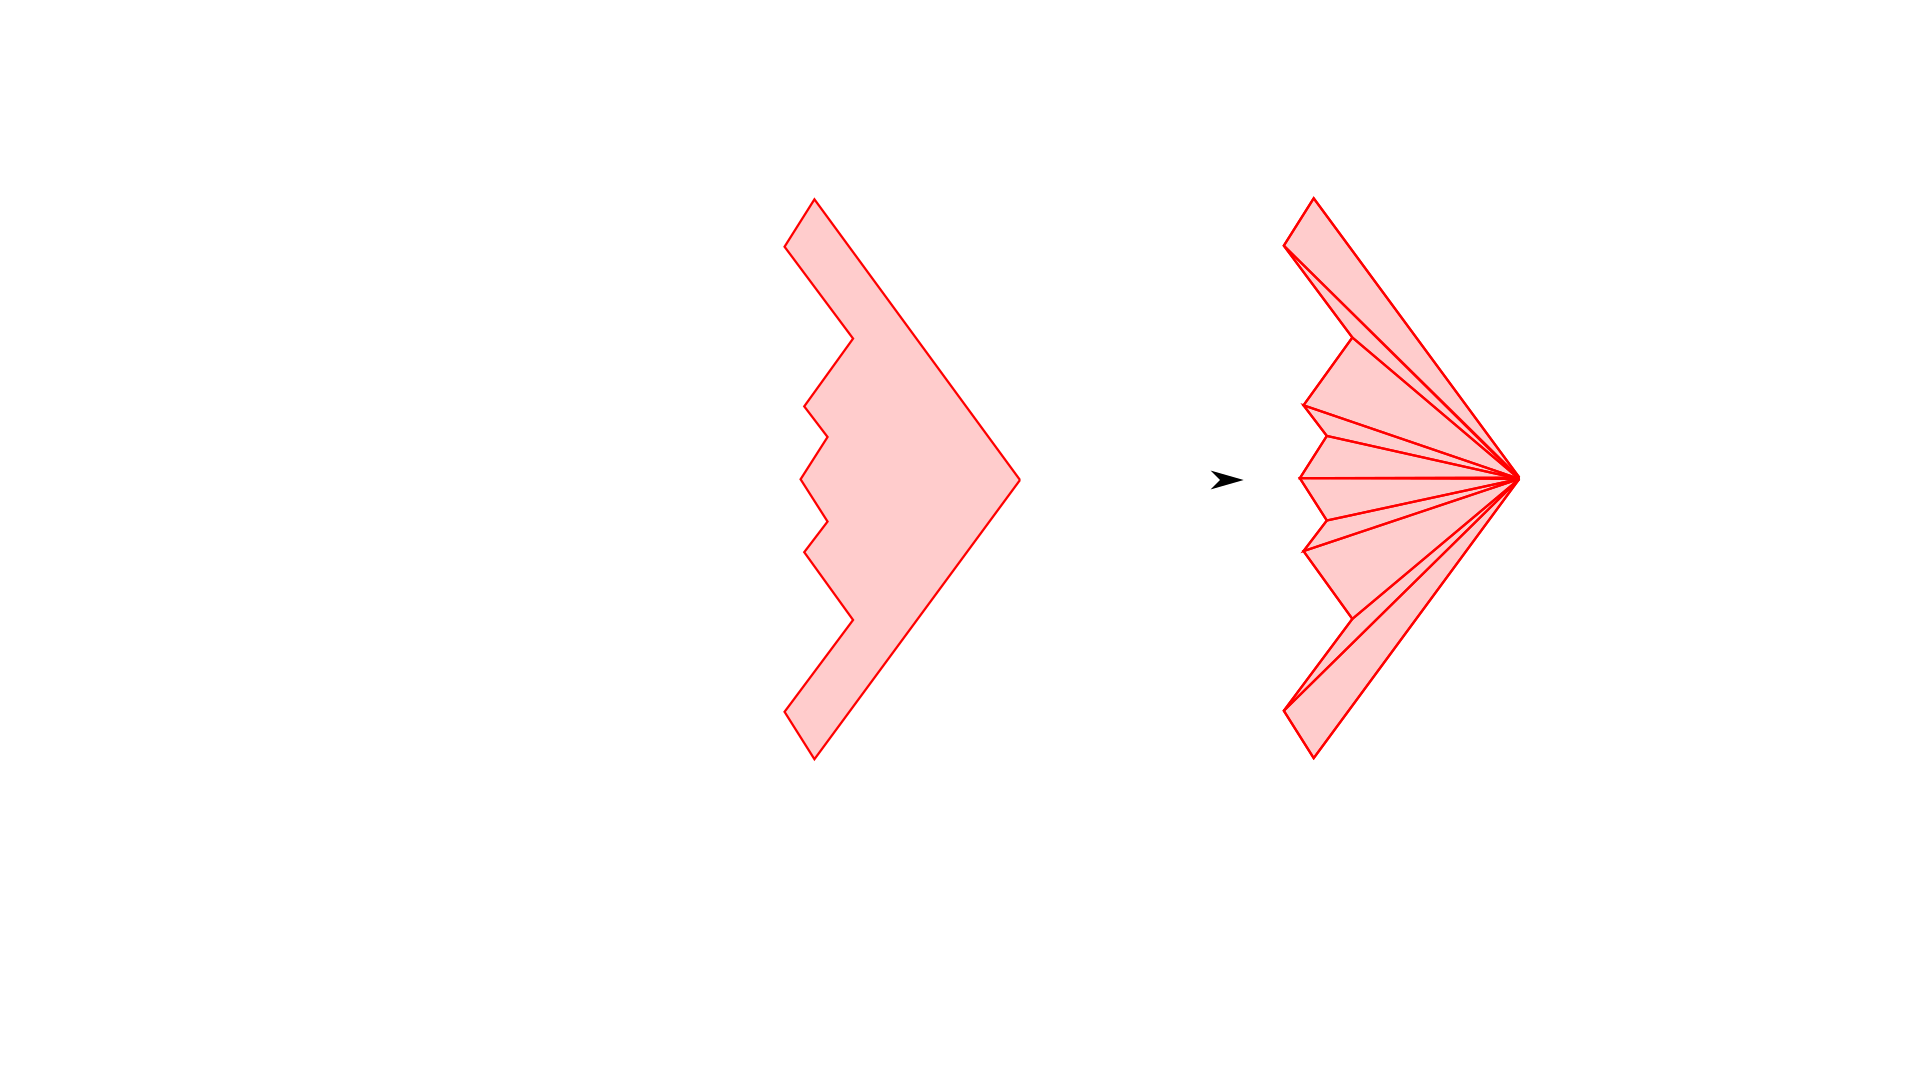
\includegraphics[width=0.9\linewidth]{Inkscape/surfaceDecomp.pdf}
	  
	  \column{0.55\textwidth}
		\small
		\vspace{0.5em}
	\pause
	\phantom{+}\newline
	  Uniform scattering distribution
	  \begin{equation*}
		\mathcal{U}(z;\widetilde{\mathcal{I}})
		= \frac{\sum_{i=1}^n \mathds{1}_{\widetilde{\mathcal{I}}_i}(z)}{\textrm{area}(\widetilde{\mathcal{I}})}
		= \sum_{i=1}^n
		\underbrace{\frac{\textrm{area}(\widetilde{\mathcal{I}}_i)}{\textrm{area}(\widetilde{\mathcal{I}})}}_{\triangleq w_{\text{s},i}} 
		\underbrace{\frac{\mathds{1}_{\widetilde{\mathcal{I}}_i}(z)}{\textrm{area}(\widetilde{\mathcal{I}}_i)}}_{=\mathcal{U}(z;\widetilde{\mathcal{I}}_i)}
	  \end{equation*}
	  	\pause
		Single point likelihood
	  	\begin{equation*}
			\mathcal{L}_{\text{s}}(\widetilde{y}|\widetilde{S})=\sum_{i=1}^n w_{\text{s},i} \underbrace{\int \mathcal{N}(\widetilde{y}-\widetilde{z};0,R)\,\,\mathcal{U}(\widetilde{z};\widetilde{\mathcal{I}}_i)\text{ d}\widetilde{z}}_{\triangleq \mathcal{L}_{\text{s},i}(\widetilde{y};R)}
		\end{equation*}

		% \pause
		% Single point likelihood (Monte Carlo)
	  	% \begin{equation*}
		% 	\begin{aligned}
		% 	\mathcal{L}_{\text{s}}^{\text{MC}}(\widetilde{y}|\widetilde{S})&=\sum_{i=1}^n w_i\left[\frac{1}{N_i}\sum_{k=1}^{N_i} \mathcal{N}(\widetilde{y}-\widetilde{z}^{(k)};0,R)\right]\\
		% 	\widetilde{z}^{(k)}&\sim \mathcal{U}(\widetilde{\mathcal{I}}_i)
		% \end{aligned}
		% \end{equation*}
	\end{columns}
	  \end{frame}
  
\begin{frame}{Tracking for general objects}
	\vspace{0.2cm}
	\begin{center}
		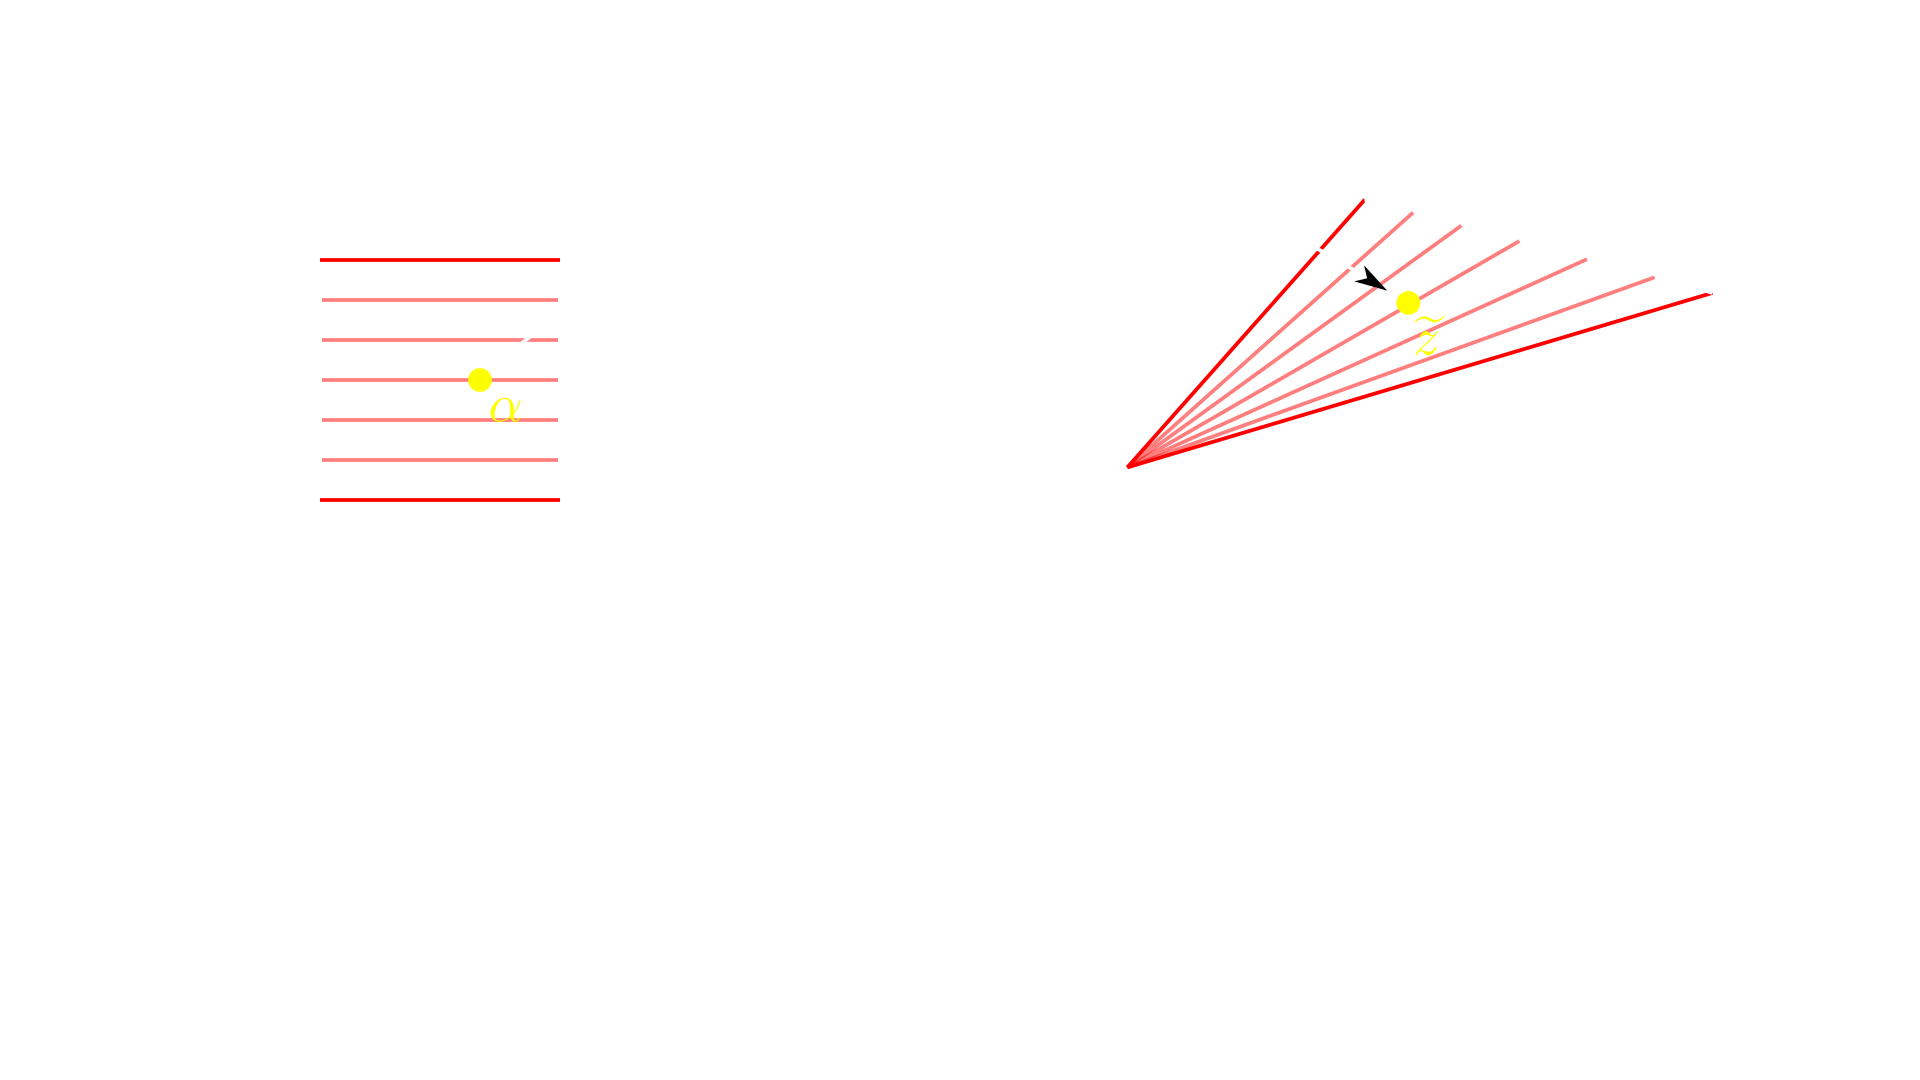
\includegraphics[width=0.8\textwidth]{Inkscape/surfaceMap.pdf}
	\end{center}
	\pause
	\vspace{0.4cm}
	\begin{equation*}
		\begin{aligned}
		\mathcal{L}_{\text{s},i}(\widetilde{y};R)&=
		\int_{[0,1]^2} \mathcal{N}(\widetilde{y}-\widetilde{\kappa}_{\text{s}}(\alpha);0,R)\text{ d}\alpha\\
		&\approx\frac{1}{N_i}\sum_{k=1}^{N_i} \mathcal{N}\left(\widetilde{y}-\widetilde{\kappa}_{\text{s}}(\alpha^{(k)});0,R\right)
		\qquad
		{\alpha}^{(k)}\sim \mathcal{U}([0,1]^2)
		\end{aligned}
	\end{equation*}
\end{frame}  

\begin{frame}{Tracking for general objects}
	Measurement model (contour)
	\begin{equation*}
	\begin{aligned}
		\widetilde y&\triangleq \widetilde{z}+v\\
		\widetilde{z}&\sim \mathcal{U}(\partial\widetilde{\mathcal{I}})\\
		v&\sim \mathcal{N}(0,R)
		\end{aligned}
	\qquad \partial\widetilde{\mathcal{I}}\triangleq \text{object contour}
	\end{equation*}
	\pause
	Single point and point-cloud likelihoods 
	\begin{equation*}
		\begin{aligned}
	\mathcal{L}_{\text{c}}(\widetilde{y}|\widetilde{S})&\triangleq\int \mathcal{N}(\widetilde{y}-\widetilde{z};0,R)\,\,\,\mathcal{U}(\widetilde{z};\partial\widetilde{\mathcal{I}})\text{ d}\widetilde{z}\\
	\mathcal{L}_{\text{c}}(\widetilde{\mathcal{Y}}|\widetilde{S})&\triangleq\prod_{j=1}^{m}\mathcal{L}_{\text{c}}\left(\widetilde{y}^{(j)}|\widetilde{S}\right)
	\end{aligned}
	\end{equation*}
	\pause
	Uniform scattering distribution
	\begin{equation*}
		\mathcal{U}(z;\partial\widetilde{\mathcal{I}})\triangleq 
		\frac{\mathds{1}_{\partial\widetilde{\mathcal{I}}}(z)}{\int_{\partial\widetilde{\mathcal{I}}}
		\text{ d}\zeta}\,\,
		\color{orange}{
		\triangleq\frac{\mathds{1}_{\partial\widetilde{\mathcal{I}}}(z)}{\textrm{length}(\partial\widetilde{\mathcal{I}})}}
	\end{equation*}
	\end{frame}

\begin{frame}{Tracking for general objects}
	\begin{columns}[c] 
		\column{0.45\textwidth}
		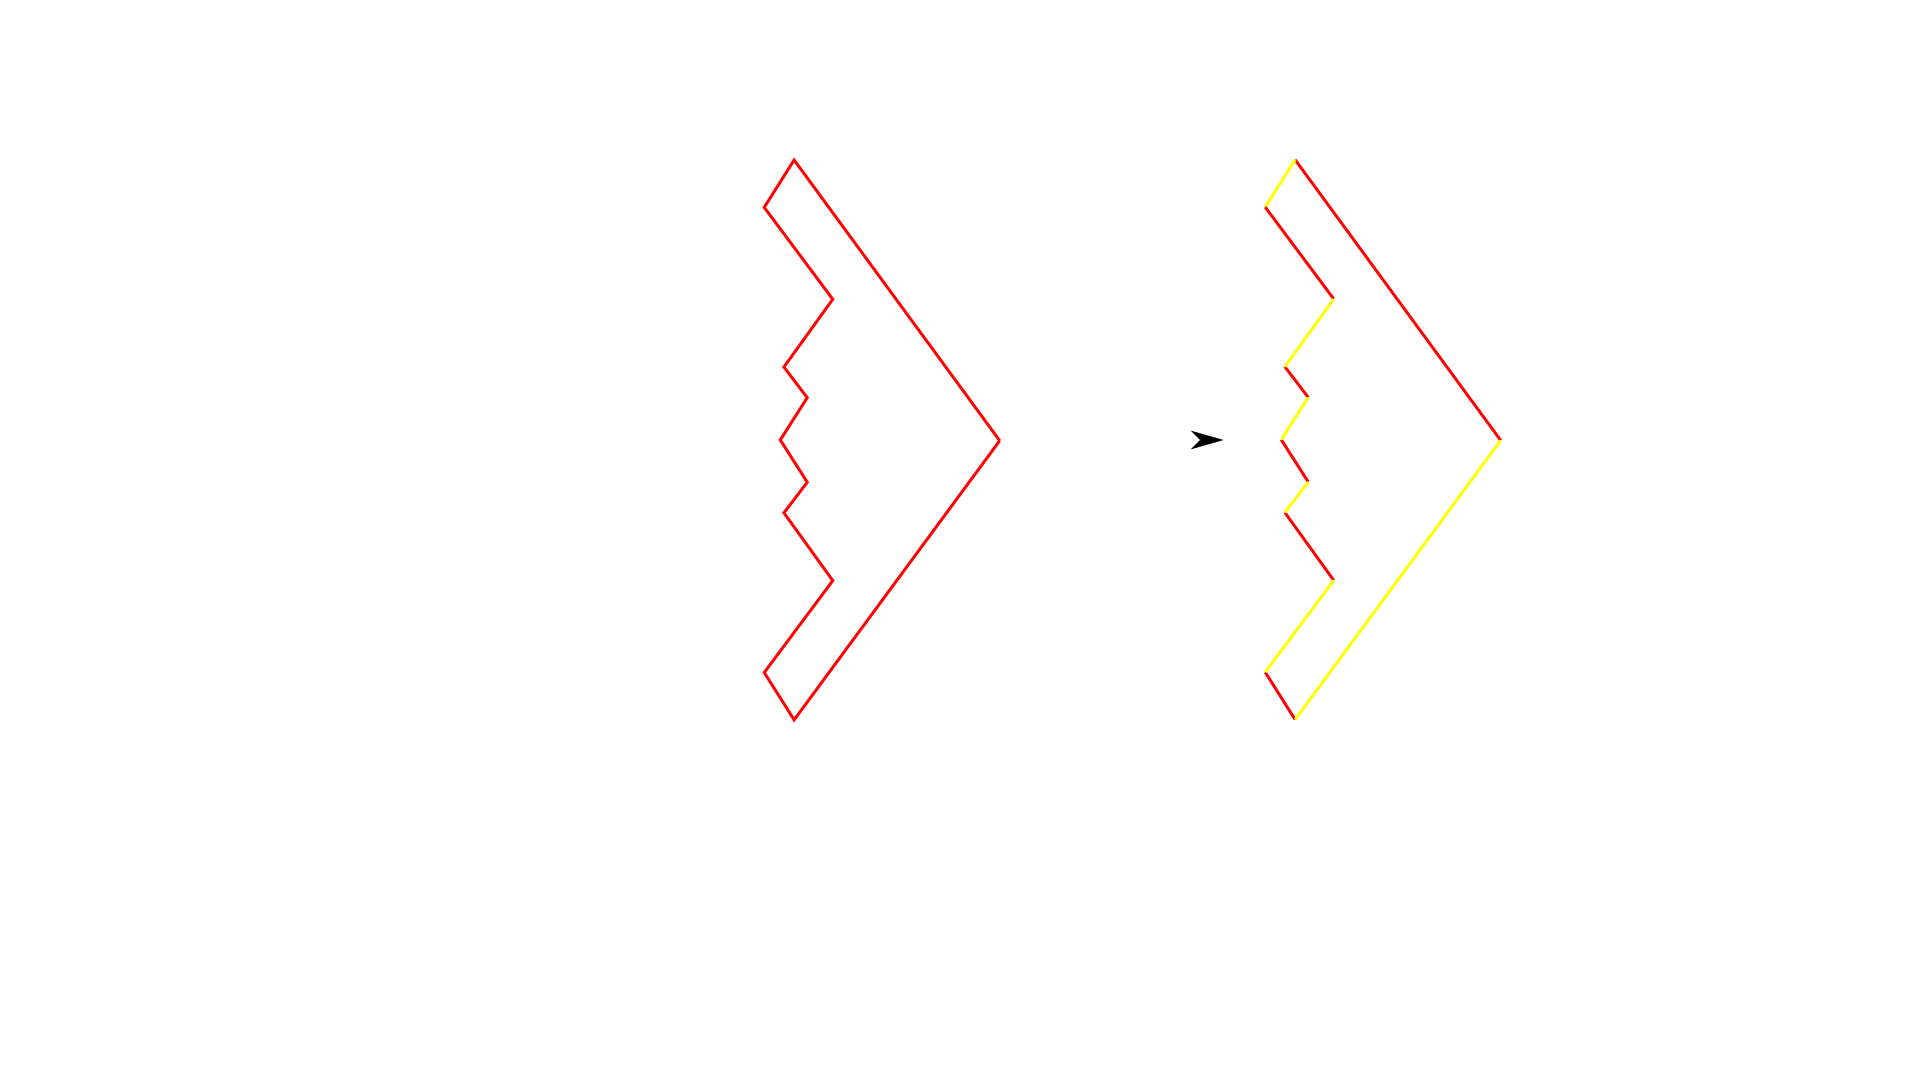
\includegraphics[width=0.9\linewidth]{Inkscape/contourDecomp.pdf}
		
		\column{0.55\textwidth}
		\small
		\vspace{0.5em}
		\pause
		\phantom{+}\newline
		Uniform scattering distribution
		\begin{equation*}
		\mathcal{U}(z;\partial\widetilde{\mathcal{I}})
		= \sum_{i=1}^n
		\underbrace{\frac{\textrm{length}(\partial\widetilde{\mathcal{I}}_i)}{\textrm{length}(\partial\widetilde{\mathcal{I}})}}_{\triangleq w_{\text{c},i}} 
		\underbrace{\frac{\mathds{1}_{\widetilde{\partial\mathcal{I}}_i}(z)}{\textrm{length}(\partial\widetilde{\mathcal{I}}_i)}}_{=\mathcal{U}(z;\partial\widetilde{\mathcal{I}}_i)}
		\end{equation*}
			\pause
		Single point likelihood
			\begin{equation*}
			\mathcal{L}_{\text{c}}(\widetilde{y}|\widetilde{S})=\sum_{i=1}^n w_{\text{c},i} \underbrace{\int \mathcal{N}(\widetilde{y}-\widetilde{z};0,R)\,\,\mathcal{U}(\widetilde{z};\widetilde{\mathcal{I}}_i)\text{ d}\widetilde{z}}_{\triangleq \mathcal{L}_{\text{c},i}(\widetilde{y}; R)}
		\end{equation*}
	\end{columns}
	\end{frame}

	\begin{frame}{Tracking for general objects}
		\vspace{0.4cm}
		\begin{center}
			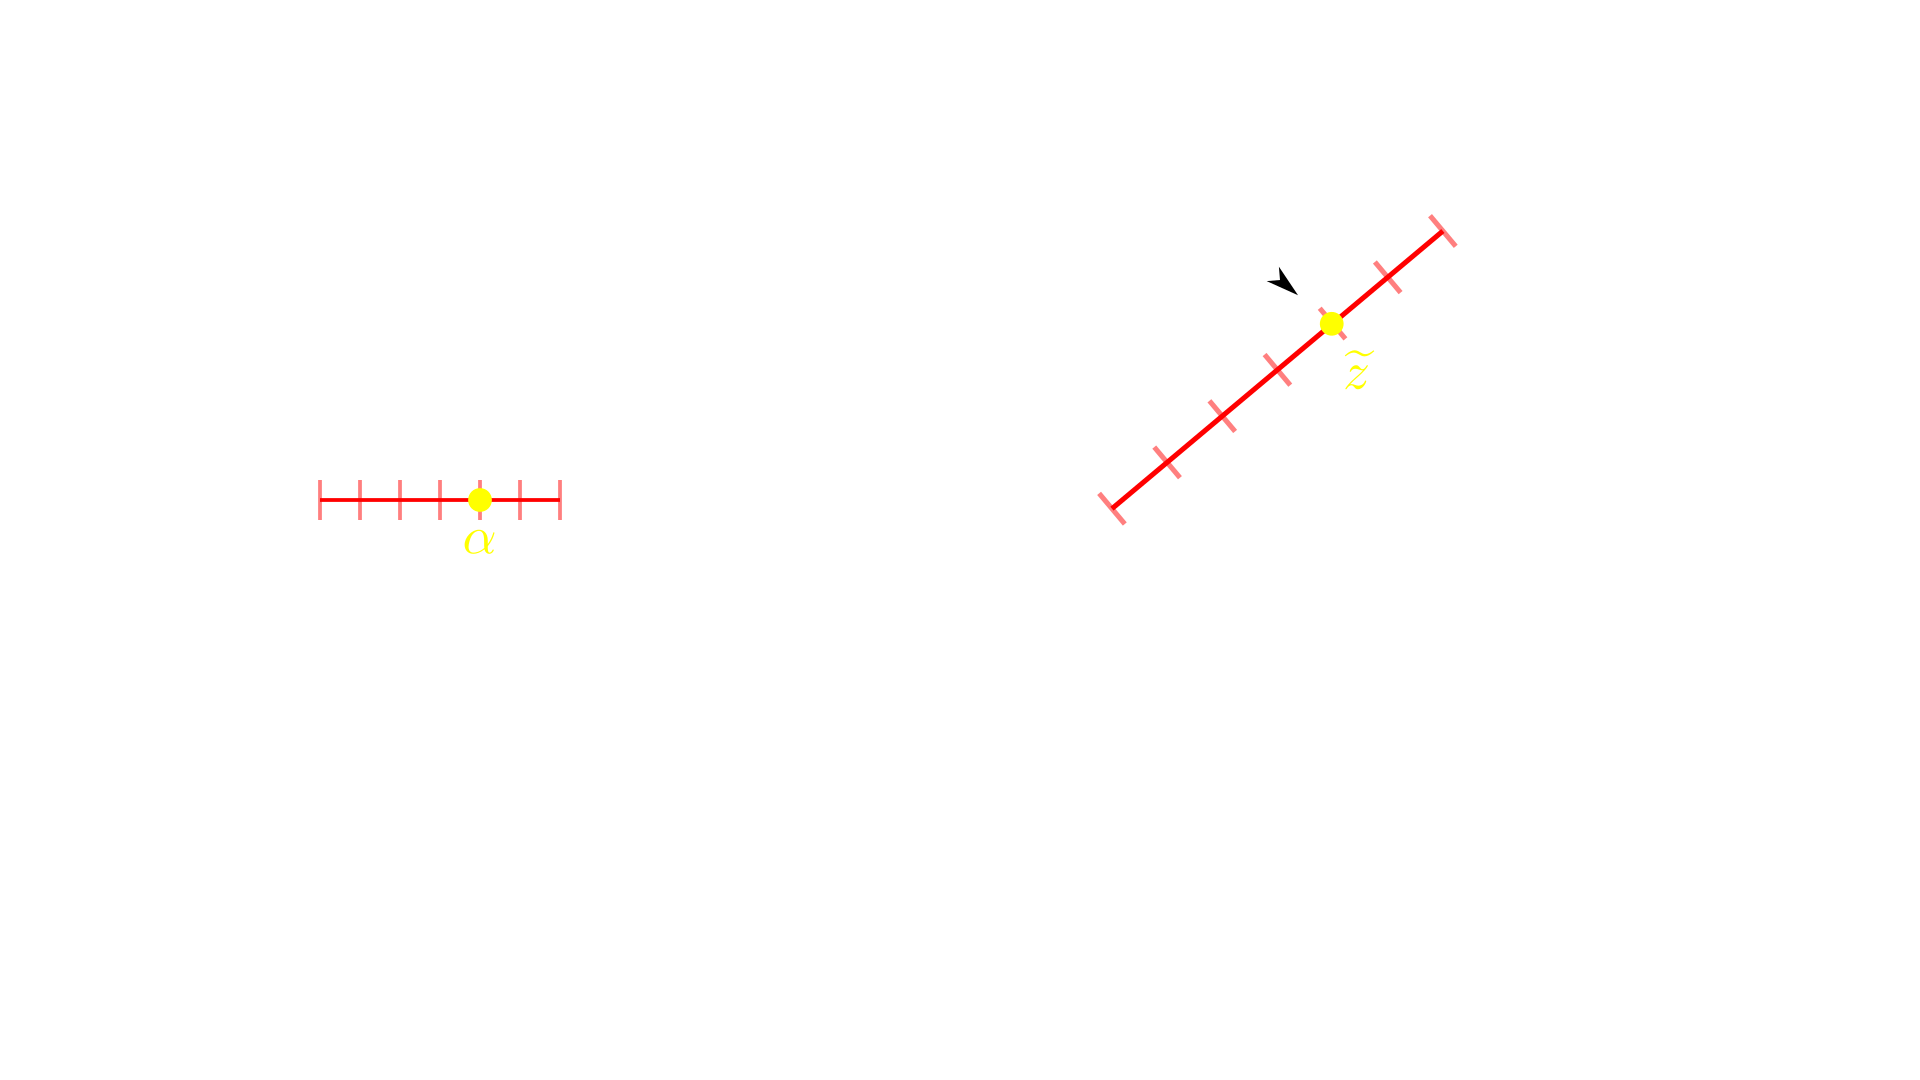
\includegraphics[width=0.65\textwidth]{Inkscape/contourMap.pdf}
		\end{center}
		\pause
		\vspace{0.4cm}
		\begin{equation*}
			\begin{aligned}
			\mathcal{L}_{\text{c},i}(\widetilde{y};R)
			&=\int_0^1 \mathcal{N}(\widetilde{y}-\widetilde{\kappa}_{\text{c}}(\alpha);0,R)\text{ d}\alpha\\
			&=\int_0^1 \mathcal{N}(A_i\alpha+B_i;0,R)\text{ d}\alpha
			\end{aligned}
		\end{equation*}
	\end{frame}  

	\begin{frame}{Tracking for general objects}
	\begin{equation*}
		\begin{aligned}
	\mathcal{L}_{\text{c},i}(\widetilde{y};R) 
	&=\int_0^1 \mathcal{N}(A_i\alpha+B_i;0,R)\text{ d}\alpha\\
	\pause
	&=\int_0^1 
	\color{yellow}{\frac{\mathcal{N}(B_i;0,R)}{\mathcal{N}\left(\frac{B_i'R^{-1}A_i}{A_i R^{-1}A_i};0,1\right)}} 
	\color{white}{\frac{\mathcal{N}\left(\alpha;\color{green}{-\frac{B_i'R^{-1}A_i}{A_i'R^{-1}A_i}},\color{orange}{\frac{1}{A_i'R^{-1}A_i}}\color{white}{}\right)}{\color{yellow}{\sqrt{A_i'R^{-1}A_i}}}\text{ d}\alpha}
	\qquad \text{(square compl.)}\\
	\pause
	&=\color{yellow}{C_i(\widetilde{y}; R)}\,\color{white}{\int_0^1 \mathcal{N}\left(\alpha;\color{green}{\mu_i(\widetilde{y};R)}\color{white}{,}\,\,\color{orange}{\sigma_i^2(\widetilde{y};R)}\color{white}{}\right)\text{ d}\alpha}\\	
	\pause
	&=\color{yellow}{C_i(\widetilde{y}; R)}\,
	\color{white}{\left[\Phi\left(\frac{1-\color{green}{\mu_i(\widetilde{y};R)}}{\color{orange}{\sigma_i(\widetilde{y};R)}}\right)-\Phi\left(-\frac{\color{green}{\mu_i(\widetilde{y};R)}}{\color{orange}{\sigma_i(\widetilde{y};R)}}\right)\right]}
		\end{aligned}
	\end{equation*}
	\vspace{0.1cm}
	\begin{center}
	[Tesori et al., 2024]
	\end{center}
	\end{frame}

\begin{frame}{Simulation}
	\begin{center}
		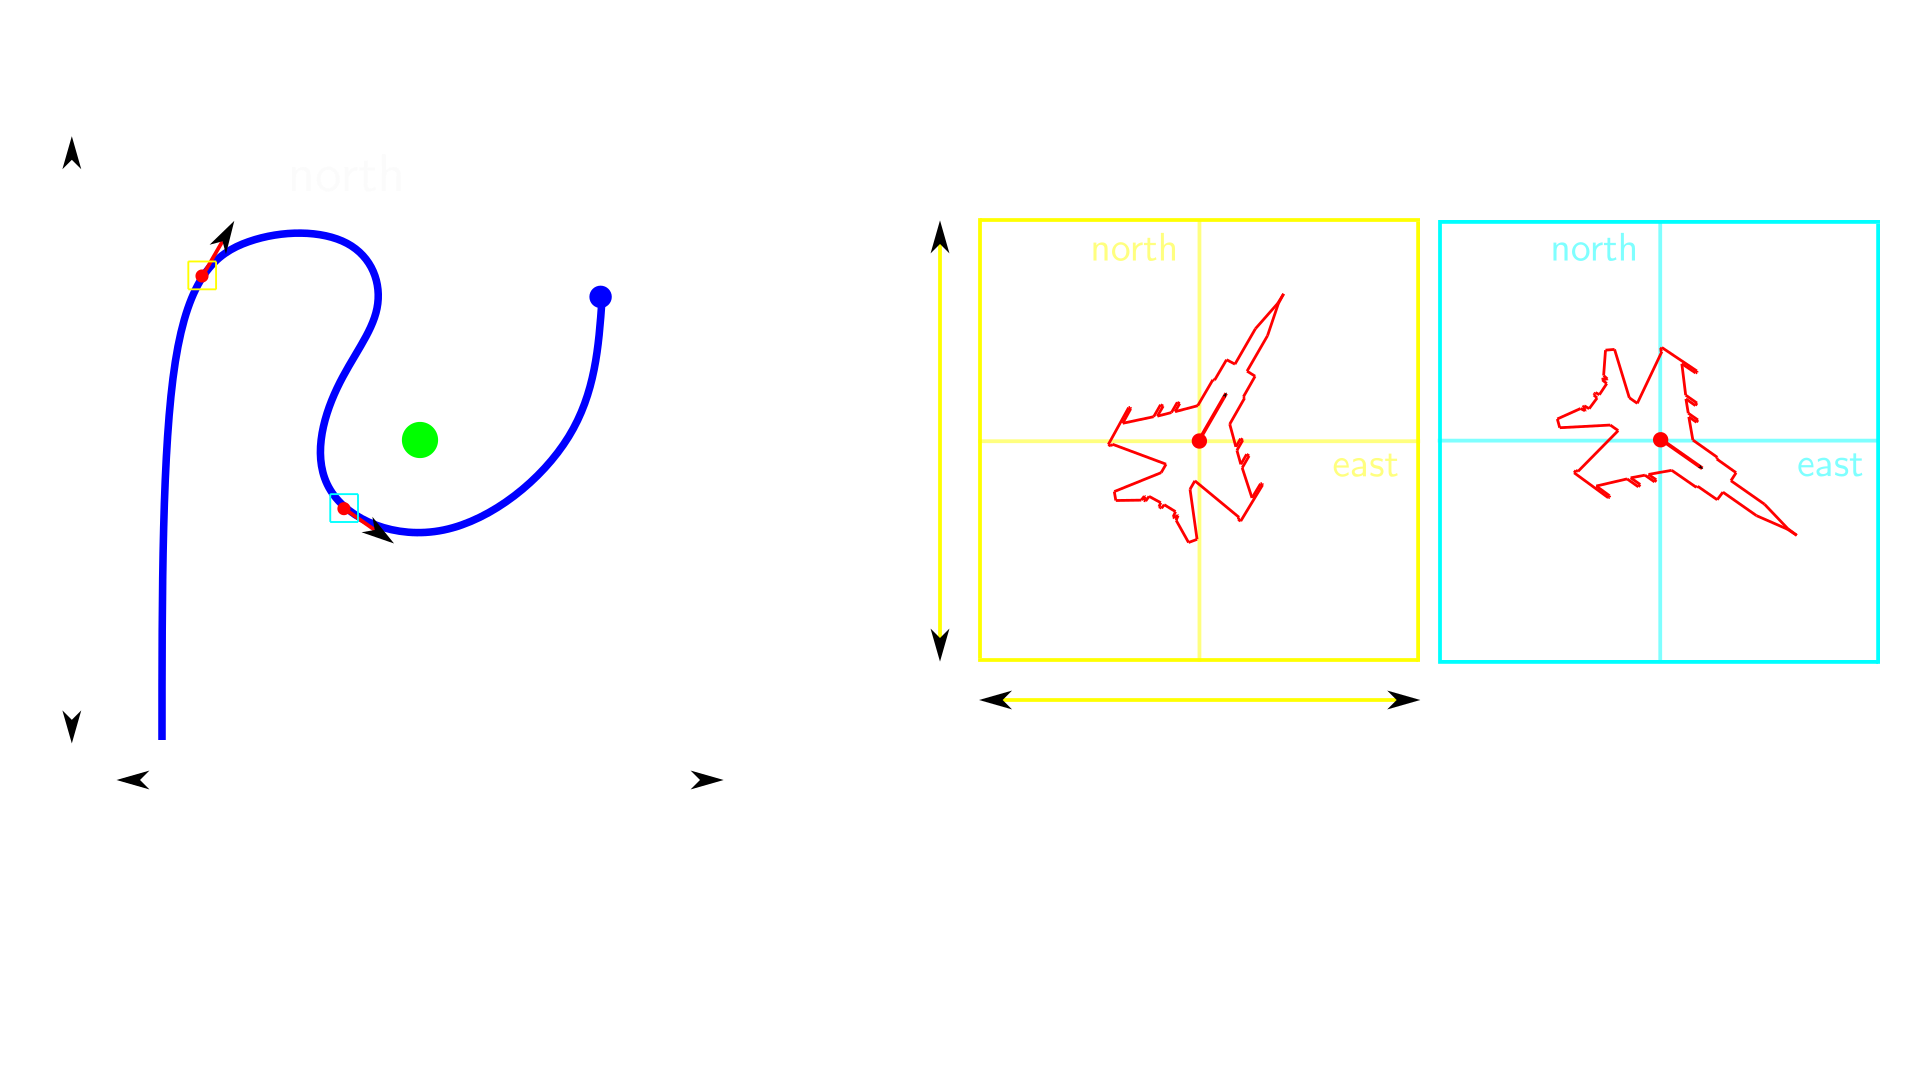
\includegraphics[width=1\textwidth]{Inkscape/groundTruth.pdf}
	\end{center}
\end{frame}

\begin{frame}{Simulation}
	\begin{center}
		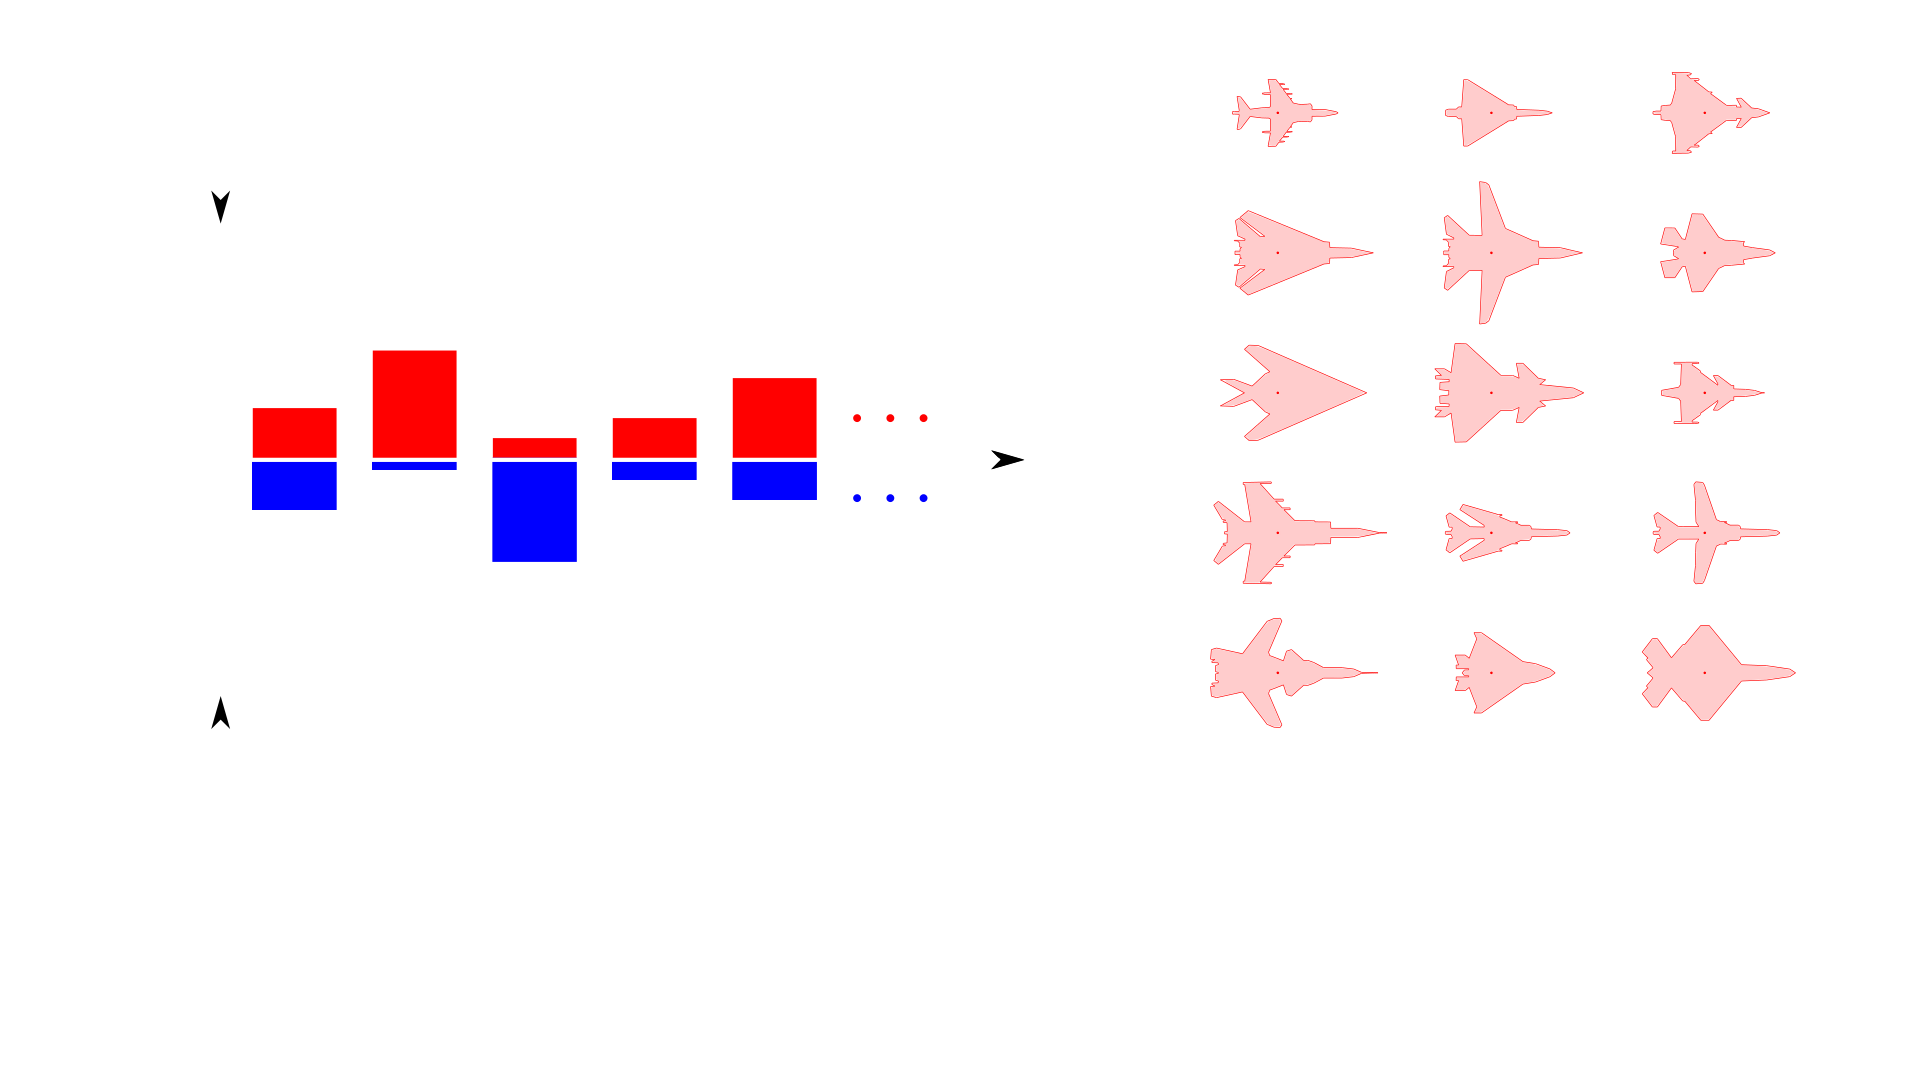
\includegraphics[width=1\textwidth]{Inkscape/shapeBelief.pdf}
	\end{center}
\end{frame}

\begin{frame}{Simulation}
	\vspace{1cm}
	\begin{center}
		\href{https://www.youtube.com/embed/WSCnlCPs1Oo?autoplay=0&start=0}{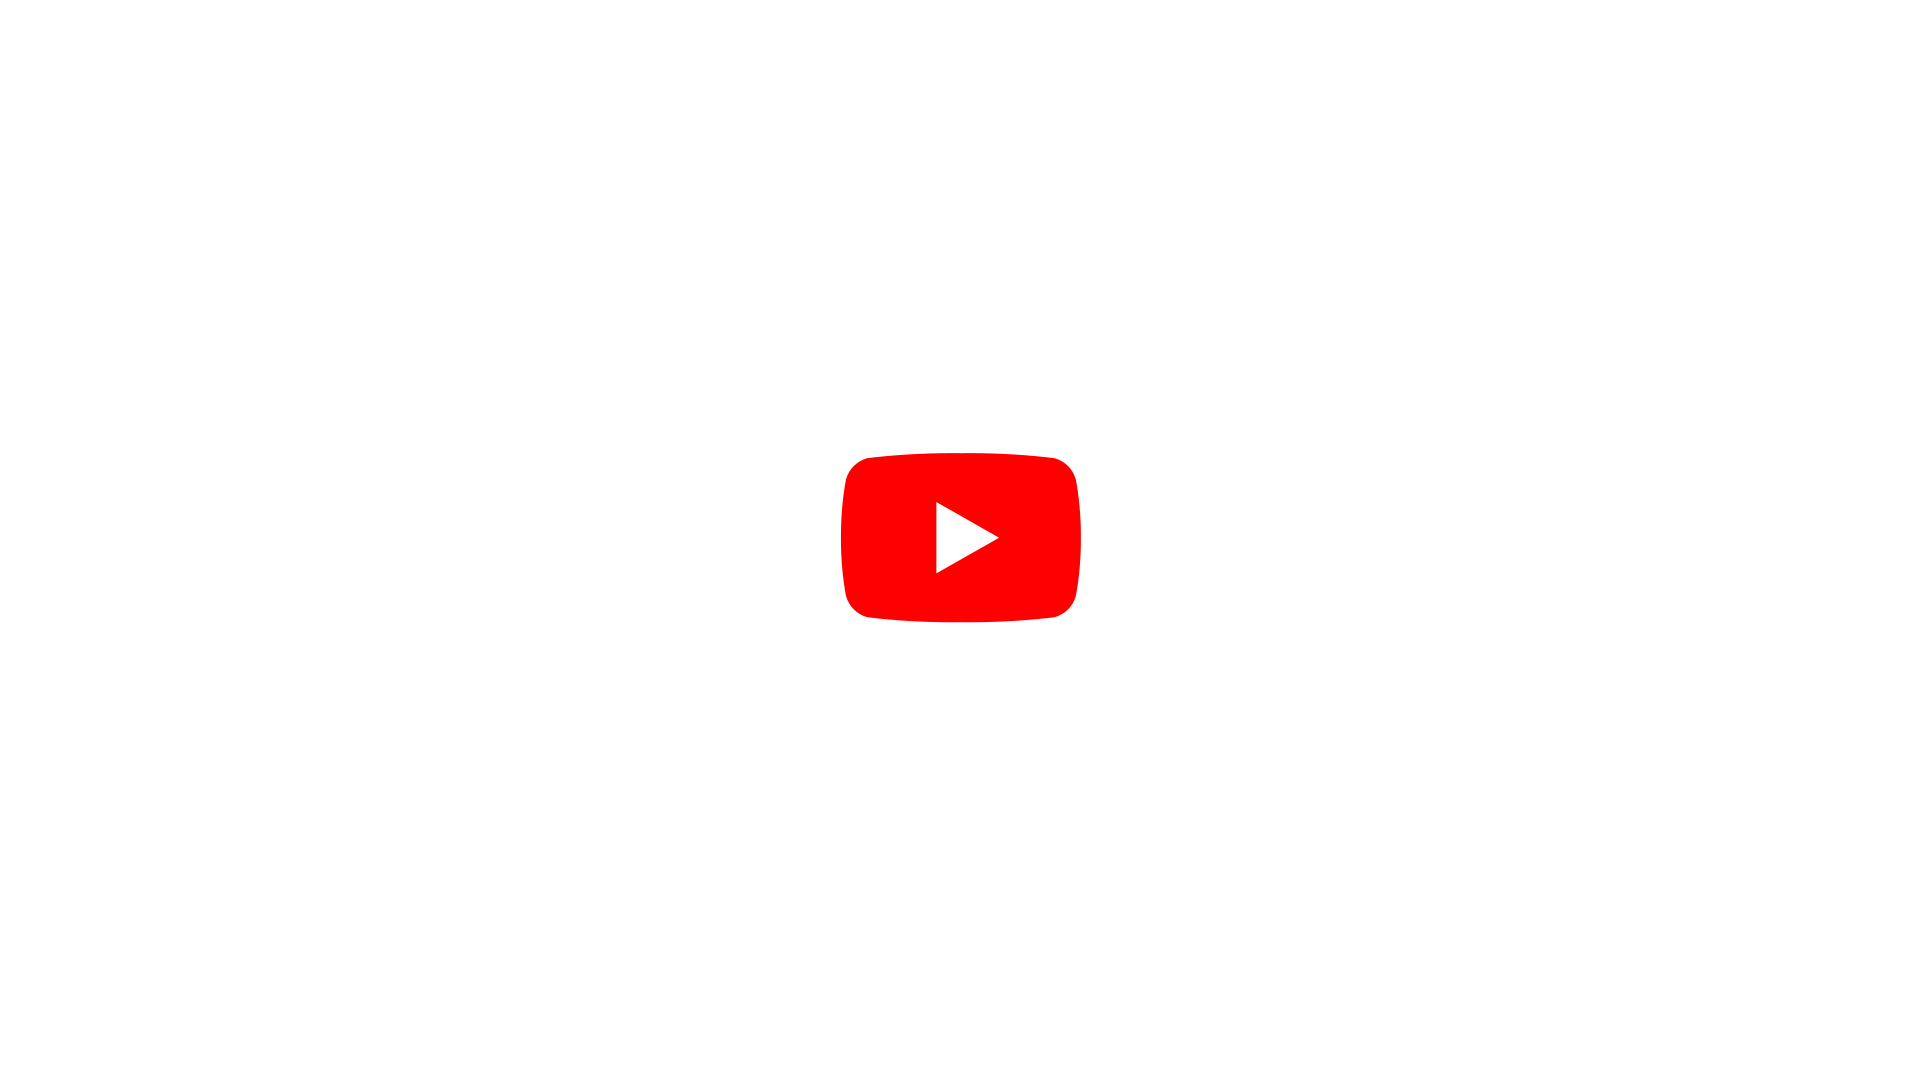
\includegraphics[width=0.15\textwidth]{Inkscape/video.pdf}}
	\end{center}
\end{frame}

\section[Conclusions]{Conclusions}

\begin{frame}{Summary}
	A solution for EOT has been presented, \textbf{taking into account the following aspects}:
	\begin{itemize}
		\pause
		\item point cloud provides information about heading;
		\pause
		\item shape is time-invariant for rigid objects;
		\pause
		\item shape does not necessarily have to be generated ex-novo.
	\end{itemize}
	\pause
	The \textbf{main limitations} of the proposed solution are:
	\begin{itemize}
		\pause
		\item accuracy significantly drops with non-uniform point clouds;
		\pause
		\item high computational cost;
		\pause
		\item shape does not affect position and heading estimation.
	\end{itemize}
\end{frame}

\begin{frame}{Outlook}
	\begin{itemize}
		\item \textbf{Direction 1:} occlusion-based EOT via ray-casting
		\pause
		\item \textbf{Direction 2:} multisensor EOT (centralized and distributed)
		\pause
		\item \textbf{Direction 3:} multi-EOT in clutter via Random Finite Sets
		\pause 
		\item \textbf{Direction 4:} agnostic shaping via MAP optimization and deep learning
		\pause
		\item \textbf{Direction 5:} 3-dimensional EOT via computer vision models
	\end{itemize}
\end{frame}

% \begin{frame}[standout]
%     %\vfill
% 	\begin{center}
%     \Huge Thank you
% 	\end{center}
% 	% \vspace{0.2cm}
%     % {\footnotesize  \textnormal{made with \twemoji{beating heart} in Florence}}\\
% 	% \vspace{-0.2cm}
% 	% {\footnotesize \textnormal{\textrm{\textcopyleft} \hspace{0.01cm} all wrong reserved}}
%     % \vfill
% \end{frame}

{\usebackgroundtemplate{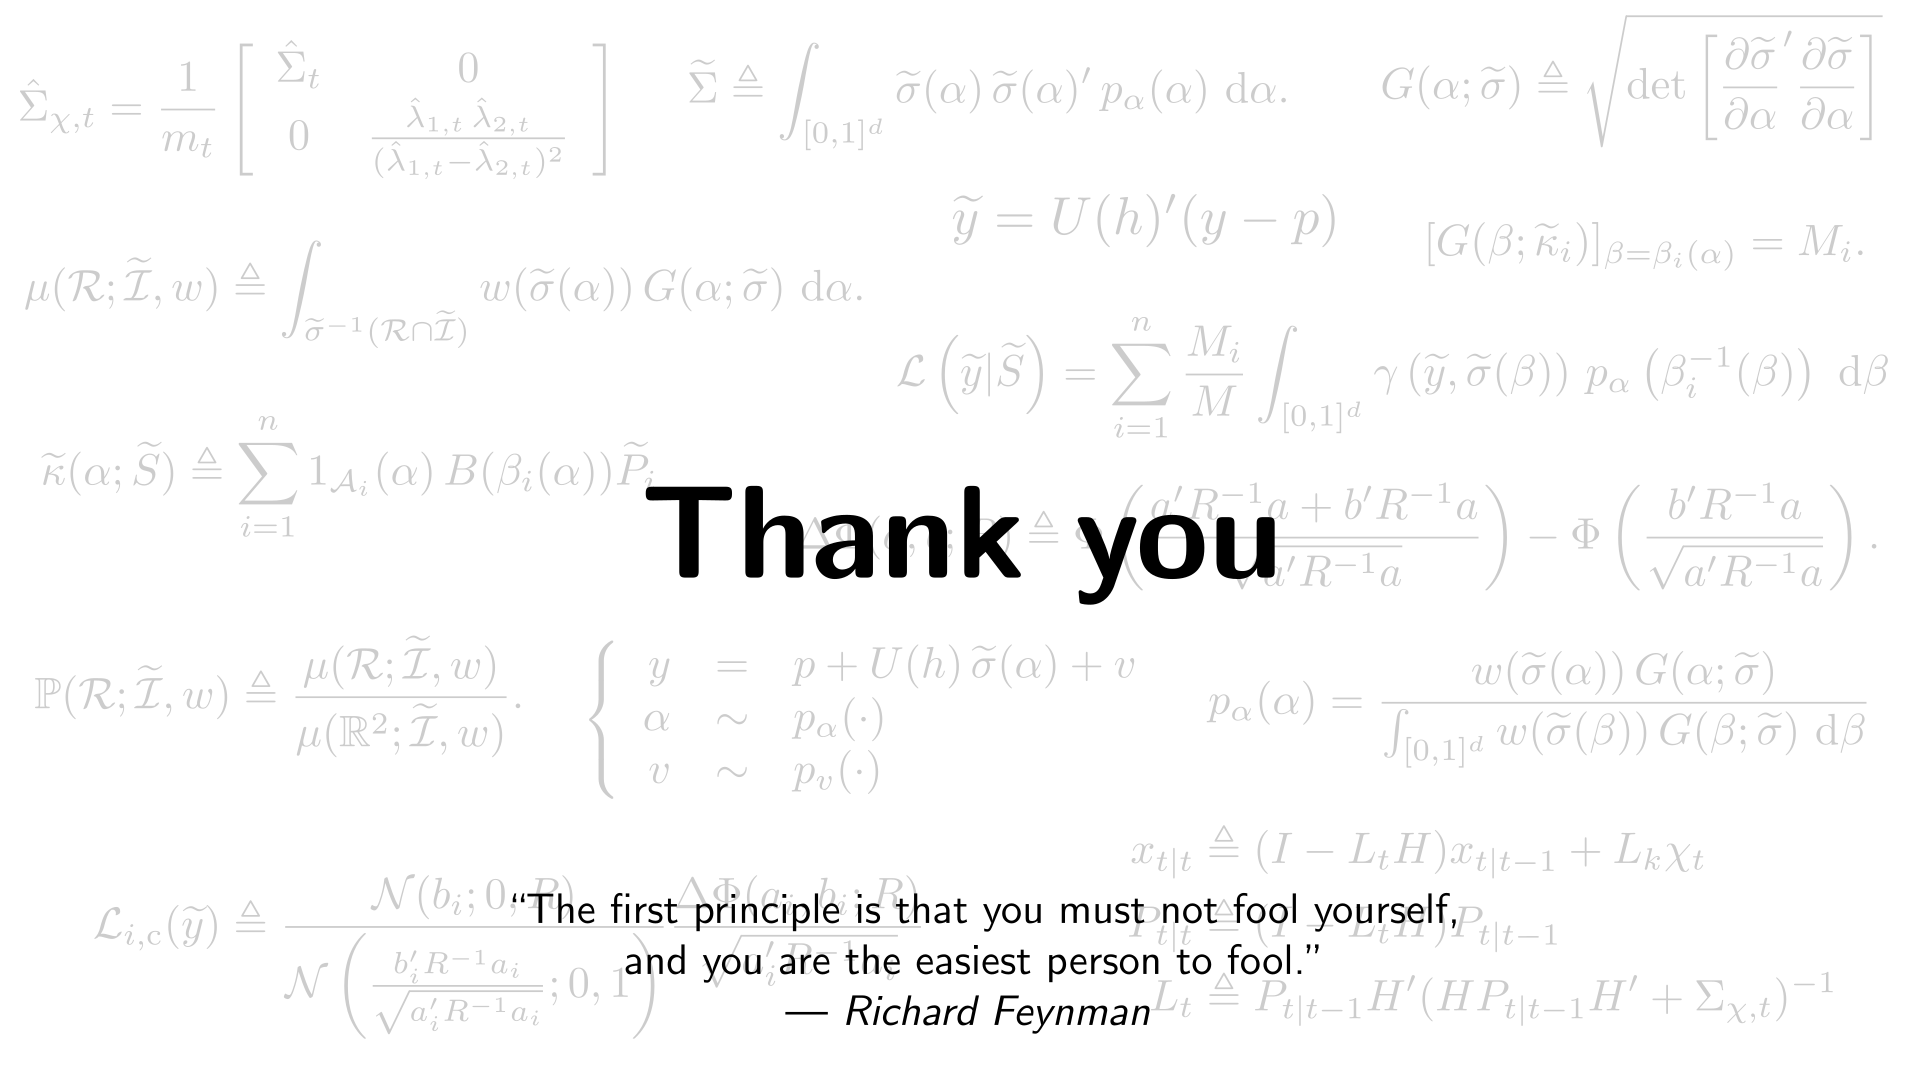
\includegraphics[width=\paperwidth]{figures/Inkscape/thanks2.pdf}}
\begin{frame}
\end{frame}}

\end{document}


